

\documentclass[11pt]{article}

\usepackage{pdflscape}
\usepackage{amsmath}
\usepackage{amssymb}
\usepackage{graphicx}
\usepackage{cite}
%\usepackage{pdfsync}

\usepackage{color} 

\usepackage{setspace} 
\doublespacing

\usepackage[round]{natbib}
%\usepackage[english]{babel}

% Text layout
\topmargin 0.0cm
\oddsidemargin 0.5cm
\evensidemargin 0.5cm
\textwidth 16cm 
\textheight 21cm

\usepackage[labelfont=bf,labelsep=period,justification=raggedright]{caption}


\makeatletter
\renewcommand{\@biblabel}[1]{\quad#1.}
\makeatother


\date{}

\usepackage{xspace}
%\usepackage{soul}
\usepackage{verbatim}
\newcommand{\etal}{{\em et al.}\xspace}
\newcommand{\var}[1]{\mathrm{Var}\left( #1 \right)}
\newcommand{\cov}[2]{\mathrm{Cov}\left( #1 , #2 \right) }
\newcommand{\se}[1]{\mathrm{SE}\left( #1 \right)}
\usepackage{lscape}
\newcommand{\beginsupplement}{%
        \setcounter{table}{0}
        \renewcommand{\thetable}{S\arabic{table}}%
        \setcounter{figure}{0}
        \renewcommand{\thefigure}{S\arabic{figure}}%
     }

\newcommand{\bcomment}[1]{{\bf{\emph{\large{[Buhm's comment:#1]}}}}}
\usepackage{bm} 



\begin{document}


\begin{flushleft}
{\Large
\textbf{An association mapping framework  to account for the sex difference in genetic architectures
}
}



    Eun Yong Kang\,$^{1,\dagger}$,
    Cue Hyunkyu Lee\,$^{5,6,\dagger}$,
    Nicholas A. Furlotte\,$^{1}$,
    Jong Wha Joo\,$^{2}$,
    Emrah Kostem\,$^{1}$,
    Noah Zaitlen\,$^{3}$, 
    Eleazar Eskin\,$^{1,4,\ast}$,
    Buhm Han\,$^{5,6,\ast}$\\
    {\bf $1$} Computer Science Department, University of California, Los Angeles, California, USA\\
    {\bf $2$} Interdepartmental Program in Bioinformatics, University of California Los Angeles, California, USA\\
    {\bf $3$} Department of Medicine, University of California San Francisco, California, USA\\
    {\bf $4$} Department of Human Genetics, University of California, Los Angeles, California, USA\\
    {\bf $5$} Asan Institute for Life Sciences, Asan Medical Center, Seoul, Republic of Korea\\ 
    {\bf $6$} Department of Convergence Medicine, University of Ulsan College of Medicine, Seoul, Republic of Korea\\ 
$\ast$ Corresponding Authors E-mails: eeskin@cs.ucla.edu, buhm.han@amc.seoul.kr\\
$\dagger$ These authors contributed equally.
\end{flushleft}

% Please keep the abstract between 250 and 300 words
\clearpage
\section*{Abstract}
% \bcomment{need some refinements}
Over the past few years, 
genome-wide association studies have identified many trait-associated loci
that have different effects on females and males,
which increased attention to the genetic architecture differences between the sexes.
%Using analyses of the North Finland Birth Cohort (NFBC) data,
%we show that 
The between-sex differences in genetic architectures can cause a 
%number of different observed 
variety of phenomena 
such as 
the differences in effect sizes at trait-associated loci,
differences in the magnitudes of polygenic background effects,
and
differences in phenotypic variances. 
%effect size differences, polygenic background effects differences,
%and phenotypic variance differences.
However, 
current approaches for dealing with sex such as including sex as a covariate
cannot fully account for these phenomena and can be  suboptimal in statistical power.
We present a novel framework, MetaSex, that can
comprehensively account for the genetic architecture differences between the sexes.
%Our framework uses a unique statistical procedure that combines a linear mixed model and a meta-analysis approach.
%to effectively account for multiple possible 
%phenomena caused by sex differences.
Through simulations and applications to real data, 
we show that our framework  has a superior performance than previous approaches.


%
%\section*{Author Summary}
%Over the past few years, 
%genome-wide association studies have identified many loci associated to human traits.
%These loci have certain effect sizes on the traits. 
%However, the effect sizes often differ between sexes; for example,
%having a variant at a locus can increase susceptibility to a disease by 2-fold in men,
%but only 1.5-fold in women. 
%Moreover, real datasets show that many other things can also differ between sexes, such as
%phenotypic variances.
%Here we propose a comprehensive framework that accounts for these 
%genetic architecture differences between the sexes
%using a unique statistical model. 


%
%are not optimized for detecting these sex-interacting effects.
%Here we present a novel framework that combines linear mixed model and meta-analysis
%to effectively identify sex-interacting effects.
%%We show that each of the statistical components of standard model can have sex differences
%%and design out method to comprehensively account for those differences.
%Our method is comprehensive in that 
%it accounts for possible sex differences
%%Our model comprehensively account for sex differences
%in all statistical components of the standard model,
%including the polygenic background effects and the random errors.
%%phenotypic mean, genetic effects, polygenic effects, and residual errors.
%Through simulations and application to the North Finland Birth Cohort data, 
%we show that our method has a superior performance compared to previous approaches.
%We also show that phenotypic variances differ by sex in many traits of real dataset,
%emphasizing that a comprehensive approach accounting for sex differences in variance components should
%be applied.




%a significant number of loci implicated in genome wide association studies 
%show differences in effect sizes of males and females.  
%There are two traditional approaches for dealing with differences in sex in GWAS. 
%The first approach is to analyze each sex separately and the second approaches is analyzing both 
%sex together using sex as a covariates. 
%Unfortunately, these approaches 
%ignores the potential for a difference in effect sizes between the two sexes and thus 
%may lead to a loss in power when sex-interacting effects are present at the loci being tested.
%In this paper, we propose a new method that is optimized for identifying genetic loci with sex-interacting effects.
%In particular, our method is designed to achieve optimal power by considering the following two scenarios.
%First, the effect size may differ by sex at the locus that we perform testing.
%Second, the small effects of causal loci over the genome can interact with sex, which can yield sex-interacting polygenic effects.
%Our approach combines linear mixed model and random effects meta-analysis to account for 
%both phenomena for an optimal analysis of sex-interacting effects in GWAS. To account for sex-interacting polygenic 
%effects, we model the interaction as a variance component in a linear mixed model. To account for sex-interacting 
%effects at the locus we test, we employ hierarchical modeling of effect sizes using random effects meta-analysis framework.
%Through simulation experiments and the analysis of North Finland Birth Cohort data, 
%we show that our method has superior performance compared to the previous approaches such as traditional sex as covariate
%approach or another meta-analysis-based approach, GWAMA.


%Over the past several years, a significant number of loci implicated in genome wide association studies 
%show differences in effect sizes for males and females.  
%The prevalence of sex-interacting effects 
%both motivates strategies for discovery of sex-interacting effects and raises questions of how to analyze 
%%complicates the analysis of 
%association studies 
%consisting of both males and females.  The traditional approach to 
%%address this issue in genome wide association 
%discover sex-interacting effects is to analyze each sex separately and the traditional 
%approach to analyze association studies consisting of both males and females
%is to include sex as a covariate in the statistical model 
%when performing association analysis.
%Unfortunately, these approaches 
%%ignores the potential for a difference in effect sizes between 
%%the two sexes and thus 
%may lead to a loss in power when sex-interacting effects are present at the loci being tested.
%%throughout the genome.
%%Furthermore, genome-wide 
%%gene-by-sex effects introduce additional background phenotypic variance, 
%%which can induce additional power loss.
%%leading to 
%%both power loss and the introduction of false positive associations.
%In this paper, we present RE+SST, a novel meta-analytic approach for the analysis of genome-wide 
%association studies consisting of both males and females.  In our approach, males and 
%females are analyzed separately and the results are combined using a random effects 
%meta-analysis approach allowing for differences in effect sizes between sexes.  We 
%show that by analyzing males and females separately, our method reduces the overall 
%variance in each study, leading to an increase in statistical power. 
%Through simulation experiments and application of Northern Finland Birth Cohort data,
%we show that the power of identifying the sex-interacting loci is dependent on 
%the effect size difference between male and female studies as well as 
%the phenotypic variance difference between male and female studies after regressing out 
%the SNP effect. 
%%Through simulations and application of 
%%our method to the 
%%Northern Finland Birth Cohort data,
%In addition, we show that our method has increased power over the traditional 
%approaches including GWAMA
%for discovering associated loci with and without sex-interacting effects while controlling for false positives.

\clearpage
\section{Introduction}


Genome-wide association studies (GWAS) have successfully identified numerous genetic loci 
associated with complex human traits. 
%Previously conducted GWAS collected samples of both male and female individuals.
In recent years, increasing attention has been paid to the sex difference in genetic architectures in GWAS. 
A number of studies have found differences in effect sizes between males and females on loci associated with traits. 
\citep{Kubo:Gut:2013,Peters:Stroke:2013,Chen:ObesRev:2013,Boraska:HumMolGenet:2012,Kostis:JAmCollCardiol:2012,Magi:GenetEpidemiol:2010,Fox:PlosGenet:2012,Porcu:PlosGenet:2013,Mason:AlcoholClinExpRes:2012,kang2014metagxe,Ohmen:JAssocResOtolaryngol:2014,Randall:PlosGenet:2013}.
In particular, a large-scale meta-analysis
 of 46 studies of anthropomorphic phenotypes 
discovered seven loci with different effects between the sexes 
\citep{Randall:PlosGenet:2013}.

It remains unclear how best to account for the sex difference in genetic architectures in association mapping.
%Traditional approaches are limited in what they can detect.
%that exist in both sexes with differing effect sizes. 
One traditional approach is to analyze each sex separately using sex-specific tests (SST). 
This approach is optimal for detecting sex-specific effects that only exist in one sex,
but is not powerful for detecting effects that exist in both sexes.
Another traditional approach is to analyze the whole sample and use sex as a covariate (CV). 
This approach is optimal for detecting effects that exist in both sexes in a constant effect size, 
but is not powerful for detecting sex-interacting effects that exist in both sexes in
differing effect sizes.

%Because this approach implicitly assumes that the effect size is the same for the two sexes, it is suboptimal for detecting sex-interacting
%effects. 

In the present study, we first enumerate three possible phenomena that can be caused by
the sex difference in genetic architectures.
%argue that the difference in genetic architecture between the sexes can cause a variety of phenomena.
One is the effect size difference between the sexes at the associated locus,
%This sex-interacting effect 
which was observed in previous studies \citep{Randall:PlosGenet:2013}.
%To achieve high power to detect sex-interacting effects, it is necessary to model
%the effect size heterogeneity in statistical testing.
Another is the effect size difference between the sexes at 
numerous loci spread throughout the genome with small effects, %. %, genome-wide loci bearing small effects.
%which we call polygenic effects.
%The aggregation of these small effects 
which can manifest as 
%This phenomenon can appear as random 
polygenic background effects that interact with sex.
%If this phenomenon occurs, it is necessary to extend the standard linear mixed model
%\citep{Kang2010,Kang:2008bx,Zhou:NatGenet:2012}, 
%which is commonly used
%to control for polygenic effects, to account for the sex difference.
The final one is the phenotypic variance difference between the sexes,
which can be caused by many factors such as sex acting as a biological environment (e.g. hormone difference)
and sex interacting with external environments (e.g. lifestyle difference). 
%Because the sex can act as a biological environment, the dispersion of the phenotypic values can also
%be affected.
%In such situations, it is necessary to model distinct error terms for the two sexes in
%the statistical model. 
In our analysis of the North Finland Birth Cohort (NFBC) dataset \citep{Sabatti:NatGenet:2009}, 
we often observed these phenomena in some human traits.
%If we do not fully account for these phenomena, 
%we may not be able to achieve optimal power from association testing.

Here, we present a novel association mapping framework, MetaSex, 
that accounts for the sex difference in genetic architectures
to effectively map associations in GWAS.
Our framework  comprehensively takes into account the three aforementioned phenomena
by
uniquely combining linear mixed model and meta-analysis.
%in order to 
%take into account the three aforementioned phenomena comprehensively.
%Our statistical model combines a linear mixed model and meta-analysis framework to account for multiple possible phenomena caused by gender differences. 
%We begin with a linear mixed model with five variance components.
Our linear mixed model includes five variance components, 
where three are for capturing sex-interacting polygenic effects
and two are for modeling distinct variances of the two sexes. 
%random effect components that illustrate the polygenic background effect difference between the sexes. 
%Remaining two variance components are random error components for each gender.
We then combine the observed effect sizes of the two sexes 
%We model effect size of each sex separately, and then combine them
using the random effects meta-analysis \citep{Han:AmJHumGenet:2011} 
that provides high power for detecting sex-interacting effects.
Because this five variance component model can be
%Although being comprehensive and powerful,
%this initial model has little utility in GWAS because fitting five variance components is 
impractically slow to be applied to millions of markers in GWAS,
%To overcome this challenge, 
we propose an approximated model that splits the problem into two optimization problems each requiring only two variance components.
%we decompose the five-variance-component model into a pair of
%two-variance-component models. The model parameters in the decomposed model have a unique mapping relationship
%to the parameters in the original model. 
%Thus, our framework based on the decomposed model provides an accurate approximation to the 
%original model 
%while being computationally efficient for GWAS.
Using simulations and real data,
we demonstrate that our framework is powerful, comprehensive, and efficient.

%Therefore, we propose a practical approximation that can expedite the framework by replacing the proposed five-variance-component model with two sets of two-variance-component models,
%where each model provides separate effect size estimate for each sex. 
%We then combine those estimates using the random effects meta-analysis framwork(RE)\citep{Han:AmJHumGenet:2011} to account for effect size heterogeneity between the sexes. 
%Using simulations and real data, we demonstrate that our method has a superior performance than previous approaches.

\section{Results}
\subsection{Overview of MetaSex}
%\subsection{Combining sex-interacting test and meta-analysis method to handle sex-interacting effects}


We first provide an overview of our proposed framework.
We constructed a toy example  
with six individuals (three females and three males).
The equation in Figure \ref{overview}A shows the components in our model for testing a single SNP. 
In this equation, vector $\bf{y}$ is the observed phenotype measurements, where 
subscripts $(f)$ and $(m)$ denote females and males.
$\mu$ denotes the phenotypic mean. 
${\bf h}$ is the sex status indicator (female = 1 and male = 0),
which is included as a covariate to account for the sex-specific phenotypic mean. 
%\hl{Eun -- please change X column 1 and 2 in Figure. Thanks!}
% Cue : I did
The first column of $\bf{X}$ is the genotype vector of the SNP, whose effect size is $\beta$.
The second column of $\bf{X}$ is the 
genotype-by-sex interaction term (SNP $\times$ $\bf{h}$), 
whose effect size is $\beta_{g \times s}$.
$\mathbf{u_g}$ is a variance component that models the polygenic background effects from the genome-wide loci that affect both sexes.
%except the testing SNP. 
Consistently to the standard linear mixed model\citep{Kang2010,Kang:2008bx,Zhou:NatGenet:2012}, 
we assume that $\mathbf{u_g}$ follows a normal distribution with mean zero and variance-covariance
matrix $\sigma_g^2 \bf{K}$ where $\bf{K}$ is the kinship matrix representing the relationship between individuals.
$\mathbf{u_{f}}$ is an additional variance component that we introduced, which represents the
female-specific polygenic effects.
We assume that $\mathbf{u_{f}}$ have mean zero and variance
$\sigma_{g,f}^2 (\bf{K}\circ \bf{hh}^T)$.
%where $K_{g \times s}$ is a block diagonal kinship matrix, that is,
%where elements representing the relationship between a male and female pair become zero.
Similarly, $\mathbf{u_{m}}$ is a variance component representing the male-specific
polygenic effects,
which have mean zero and variance
$\sigma_{g,m}^2 (\bf{K}\circ \bf{(1-h)(1-h)}^T)$.
We then modeled separate error terms for females and males, assuming that error variances can be different.
$\mathbf{e_f}$ is a female-specific error term that follows a normal distribution with mean zero and variance $\sigma_{e,f}^2(\bf{I\circ hh^T})$, 
where $\bf{I}$ is the identity matrix. 
%a modified identity matrix that has ones for females in the diagonal and zero for others.
Similarly, $\mathbf{e_m}$ is a male-specific error term that have mean zero and variance $\sigma_{e,m}^2(\bf{I \circ (1-h)(1-h)^T})$.
%$e$ is the standard random error term that follows a normal distribution with mean zero and variance $\sigma_{e}^2 I$.
%$e_s$ is an additional random error term to account for sex-specific errors, 
%and is assumed to follow
%a normal distribution with mean zero and variance $\sigma_{e_m}^2 I'$,
%where $I'$ is the same to $I$ but the latter three diagonal elements are zero.

Applying this full model to GWAS can be computationally challenging 
because there are five variance components to fit ($\mathbf{u_g}$, $\mathbf{u_f}$, $\mathbf{u_m}$, $\mathbf{e_f}$, and $\mathbf{e_m}$).
Currently available linear mixed model methods for association mapping are optimized for models with two variance components \citep{Zhou:NatGenet:2012,Kang2010,Kang:2008bx}.
If there is a third component, a state-of-the-art association mapping method uses a simple grid search \citep{Lippert:NatureMethods:2011}. 
Thus, fitting five variance components may require a three-dimensional grid search, which can be prohibitively slow for GWAS.

To expedite the application of our model to GWAS, we propose an efficient decomposition of the model.
Suppose that we restrict our scope to individuals of one sex.
Then, the full model with five variance components collapses into a sex-specific model with two variance components (Figure \ref{overview}B).
%This is because 
%$\bf{K}$ and $\bf{K}\circ \bf{hh}^T$ have the same form for the female individuals.
%Similarly, we also assume that we only have a subset of individuals that are males.
%This gives us a male-specific linear mixed model with two variance components.
Thus, the model can be efficiently solved using existing approaches \citep{Zhou:NatGenet:2012,Kang2010,Kang:2008bx}.
%The key intuition is that by solving two sex-specific models separately,
%we can automatically account for the between-sex differences in phenotypic mean as well as error variances.
In the decomposed model, 
%This approximation differs from the original model in that 
we cannot
distinguish the whole-sample polygenic component ($\sigma^2_g$) from the sex-specific polygenic components ($\sigma^2_{g,f}$ or $\sigma^2_{g,m}$),
because they follow the exactly same distribution conditioned on one sex.
However, this distinction is unimportant for association mapping, 
because we anyhow want to control for both. 
%However, for the purpose of association testing, distinction of these is unimportant;
%as long as the estimate of the summation (e.g. $\sigma^2_g+\sigma^2_{g,f}$ for females) is accurate, the association results are the same.
%However, if the sample size of each sex is large enough, we expect that the loss of information will have minimal impact.

%%If we choose to ignore $\mathbf{u_g}$ for a moment, we could decompose the model into two sex-specific models (Figure \ref{overview}B).
%%Then, in each model, we can put $\mathbf{u_g}$ back. 
%As a result, we approximate the original model by using two sets of linear mixed models with two variance components,
%for which efficient optimization methods are available.
%%An optimization technique for two-variance-components models are already known and were efficiently applied to genome-wide scales \citep{Kang2010}.
%The difference in the phenotypic mean of the two models ($\mu_f$ and $\mu_m$) accounts for the sex-specific mean difference $\mu_s$.
%The difference in genetic effects ($\beta_f$ and $\beta_m$) accounts for the sex-interacting genetic effect $\beta_{g \times s}$.
%The polygenic component in each model ($\mathbf{u_f}$ and $\mathbf{u_m}$) accounts for both the polygenic and sex-interacting polygenic effects ($\mathbf{u_g}$ and $\mathbf{u_{g \times s}}$).
%Finally, the random error terms ($\mathbf{e}$) in the two models are not required to have the same variance,
%which accounts for the different random error variances of $\mathbf{e_{f}}$  and $\mathbf{e_m}$. 
%
%The difference in this approximation compared with the original model is that
%the maximum likelihood estimates of $\sigma^2_g$ and $\sigma^2_{g \times s}$ can be different between 
%the two sexes, which would not occur in the original model.
%Also, the between-sex elements of $K_g$ are ignored, which can give additional information for estimating parameters.
%However, if the number of individuals of each sex is large enough, $\sigma^2_g+\sigma^2_{g \times s}$ estimates
%($\sigma^2_f$ and $\sigma^2_m$) %$\sigma_m$ and $\sigma_f$ estimates 
%will be sufficiently accurate enough in each sex.
%%even if
%%we use only within-sex information in the approximated model.

Finally, given the sex-specific effect size estimates and the standard errors,
%from the two-variance-component model 
%male estimate and female estimatean effect size estimate and its standard error 
%from each sex-specific model 
($\hat{\beta_m}$, se($\hat{\beta_m}$), $\hat{\beta_f}$, se($\hat{\beta_f})$), we apply a series of statistical tests.
We first apply SST, 
which is optimal for detecting sex-specific effects.  
%Because it is a common practice that
%investigators look at each sex separately first, %without noticing that they are performing multiple testing.
%we explicitly include SST in our framework to account for multiple testing.
%We first test each sex separately (sex-specific test, SST) to detect sex-specific effects.
Then, to effectively detect sex-interacting effects, 
we combine the two sex-specific estimates %using meta-analysis. %information from the two sexes.
%There can be different approaches for doing this; for example, one can combine chi-square
%statistics of two sexes as is done in GWAMA \citep{Magi:GenetEpidemiol:2010}.
%We apply 
using the random effects meta-analysis method (RE) \citep{Han:AmJHumGenet:2011} (Figure \ref{overview}C),
which explicitly models heterogeneity. % and has high power.
%In this approach, the two effect sizes are assumed to come from the same underlying distribution, 
%thus modeling both the similarities and differences of them. 
%As shown below, this approach turns out to be powerful for detecting sex-interacting effects.
As a result, our framework involves three tests (Female SST, Male SST, and RE),
requiring multiple testing correction. 
%the significance threshold must be adjusted in order to account for multiple test.  
A powerful multiple testing strategy can be to adjust the significance threshold for each test 
to maximize power while controlling for overall false positive rate \citep{Eskin:GenomeRes:2008}.
We identify and propose 
%We perform extensive null simulations to identify
a set of thresholds for the three tests, what we call smart thresholding,
that exactly controls the false positive rate to the GWAS threshold ($5\times10^{-8}$) while maximizing power.

%Since the proposed approach involves performing three association tests at each locus, 
%the significant threshold must be adjusted in order to take into account these multiple tests.  One such way is to use the 
%Bonferroni correction that uses
%the significance threshold of $1.67 \times 10^{-8}$ instead of the traditional threshold of $5 \times 10^{-8}$,
%but this can be overly conservative due to correlations of tests.
%%Since the tests are correlated, this can be overly conservative. 
%We perform extensive null simulations to identify
%the threshold that exactly controls the false positive rate.
%Moreover, we choose to define different significant thresholds for SST and RE to increase power
%while still controlling for overal false positive rate,
%a strategy we call smart thresholding.
%To control false positive rate to $5 \times 10^{-8}$,
%we found that using unequal thresholds 
%$2.41 \times 10^{-8}$ for RE and $1.36 \times 10^{-8}$ for SST gives us better power.

\subsection{Power simulations}




%\subsubsection*{Power comparison design}

%Random-effects meta-analysis is not the only possible meta-analysis method that can be used in a meta-analytic approach for handling sex-interacting effects.
We performed simulations to evaluate the power of our MetaSex approach. 
Below, we also refer to our MetaSex method as RE+SST 
because the framework involves simultaneous testing of RE and SST.
%both random effects model meta-analysis (RE) and sex-specific test (SST).  
%\citep{Han:AmJHumGenet:2011} 
We compared our method to two other approaches:
%the fixed-effect meta-analysis method (FE) and
(1) CV, the traditional approach using sex as a covariate, 
 and (2) GWAMA \citep{Magi:GenetEpidemiol:2010}, another meta-analysis approach designed to discover 
sex-interacting effects.
Because CV and GWAMA are methods using the whole sample similarly to RE, 
we assumed the 
common practice in which investigators examine each sex separately using SST regardless of which method is used for the whole sample.
Thus, we compared the power of our MetaSex (RE+SST) approach with that of CV+SST and GWAMA+SST,
where A+B denotes a combination method that calls a result significant 
if either A or B method gives a significant result
after correcting for multiple testing.
%where we correct for the multiple testing. % burden using numerous null simulations.
We also compared the power of the bare SST to get a sense of how much power is increased by the methods using the whole sample.

To make a fair comparison between these methods, 
we corrected for multiple testing within each method 
%multiple testing has to be corrected 
in an equitable way. 
In MetaSex (RE+SST), CV+SST, and GWAMA+SST, we performed three tests, 
whereas in SST, we performed two tests.
Therefore, for each of these methods,
we generated 10 billion ($10^{10}$) null male/female statistic pairs 
and chose the 500th smallest p-value, which was the method-specific
significance threshold to control the false positive rate (family-wise error rate) to $5\times10^{-8}$.
The resulting significance thresholds were
%$1.67 \times 10^{-8}$ for FE+SST, 
$1.70\times10^{-8}$ for CV+SST, 
$1.73\times10^{-8}$ for GWAMA+SST, 
and $2.49\times10^{-8}$ for SST.
For MetaSex (RE+SST), we used our smart thresholding strategy that applied
$2.41 \times 10^{-8}$ for RE and $1.36 \times 10^{-8}$ for each of the two SST (see Methods).
These empirically calculated thresholds ensured that the false positive rates of all compared methods
were well controlled.
See Methods for the further details of our power simulations.
%As a result, the false positive rates of all compared methods below were appropriately controlled.
%still controlling the overall false positive rate to $5 \times 10^{-8}$ (see Methods).  
%Therefore, all methods compared below have the correct family-wise error rate.

%For RE+SST, FE+SST and GWAMA+SST, since we are performing 3 tests at each locus, 
%we use the significance threshold of $1.7 \times 10^{-8}$.  For SST, since we are performing only 2 tests at each locus, 
%we use the significance threshold of $2.5 \times 10^{-8}$.  
%
%For GWAMA, since we are performing only 1 test at each locus, we utilize the significance threshold of $5 \times 10^{-8}$. 
%We compare the statistical power of simple sex-interacting test (SST) and combining sex-differentiated 
%(RE, GWAMA) approaches and sex-interacting (SST) while varying effect size ratios between 
%male and female studies. 
%
%
%To evaluate power, we generated 10,000 case and 10,000 control individuals in the male study 
%with a relative risk of 1.1, a disease prevalence of 0.001 and a minor allele frequency of 0.1. 
%We also generated the female study with the same parameters. 
%We then decreased the effect size ratio between the 
%male and the female studies to compare the power.
%

\subsubsection*{Simulating the sex difference in effect sizes}

%We performed two power simulations. 
In the first power simulation, 
we simulated the effect size difference between the sexes,
a phenomenon called ``effect size heterogeneity''.
%We assumed that the error variances were the same for the two sexes.
%In the second simulation below, we assumed the opposite.
%Our purpose was to separate the two factors that may affect the power
%and to evaluate them independently.
We assumed a SNP of minor allele frequency 0.3 and generated genotypes of 5,000 males and 5,000 females.
Then we simulated continuous phenotypes of these individuals while assuming the same error variance
for the two sexes.
For each male individual, we generated a phenotype assuming a genetic effect size of 0.192 and variance of 1.0.
For each female individual, we generated a phenotype assuming 10\% of the male effect size (0.019) and variance of 1.0.
We repeated this simulation 1,000 times and computed the power of a method as the proportion of simulations
in which the test p-value was 
more significant than the given significance threshold. 
We then gradually increased the female effect size from 10\% to 100\% of the male effect size,
to simulate differing levels of heterogeneity.

%After we fix the male and female effect size to be 0.192 and 
%we repeat the whole procedure as we gradually decrease female effect size from 0.192 to 0.0195
%(0.1923, 0.1731, 0.1539,  0.1347, 0.1155,  0.0963,  0.0771, 0.0579,  0.0387,  0.0192)
%to simulate sex-specific effect.
%\hl{Hi Eun, can you elaborate more? What's the effect size? What's the error term variance that we assumed?}


%
%
Figure \ref{power_four} shows the power of the four approaches 
(RE+SST, CV+SST,
%, FE+SST
GWAMA+SST, and SST) with respect to the effect size ratio between the two sexes.
% in the balanced study (a) and the unbalanced study (b).
%In the balanced study, the number of individuals are equivalent between male and female ($N_{female} = N_{male}$).. 
%However in the unbalanced study, the number of individuals in female study is twice as the number of 
%individuals in male study ($N_{female} = 2N_{male}$).
%
As expected, when the effect size ratio was very small (e.g., 0.1), meaning 
that the effect is almost sex-specific,
%that effect sizes of the male and female
%studies are extremely different, 
SST showed the highest statistical power. 
As the effect size of the female study increased, the MetaSex (RE+SST) approach showed the highest statistical power,
demonstrating that our approach can effectively detect sex-interacting effects.
%both GWAMA+SST and SST approaches. 
%
%In the balanced study (Figure  \ref{power_four}(a)), when the effect size ratio is extreme (e.g. 0.1), meaning that the effect size in female study 
%is 10 times larger than male study, SST outperforms all other methods. 
%However, in all other effect size ratios, RE+SST outperforms all other methods. 
%In unbalanced study (Figure  \ref{power_four}(b)), 
%in all effect size ratios, RE+SST outperforms all other methods in terms of statistical power. 
%We provide a more detailed power analysis of the different meta-analysis methods in the supplementary.  
Even at the ratio of 1.0, a situation that the effect size was identical for both sexes (no heterogeneity),
where CV was expected to be the most powerful,
MetaSex (RE+SST) slightly outperformed CV+SST. 
This was because of our smart thresholding strategy that allowed a more liberal significance threshold for RE
with the expense of 
a more stringent threshold for SST.
%in our RE+SST approach, 
%which gives power advantage compared to CV+SST where the same significance threshold is applied to CV and two tests of SST.

\subsubsection*{Simulating the sex difference in error variances}

In the second power simulation, we simulated the error variance difference between the sexes
while assuming a constant effect size (no heterogeneity). 
%In this simulation, we assume that there exists inherent phenotypic error, which we 
%cannot capture with genetic effect and the standard error term ${\bf e}$ that follows a normal 
%distribution with mean $0$ and variance $\sigma_e^2$. 
As in the first simulation, 
for each male and female individual, we generated a phenotype assuming a genetic effect size of 0.2
%\hl{$\leftarrow$ Please fill in this number} 
and variance of 1.0.
Then, we gradually increased the error variance of the females from 1.0 to 4.0 
(standard deviation from 1.0 to 2.0).
Figure \ref{power_res} shows the power of the four approaches 
(RE+SST, CV+SST,
%, FE+SST
GWAMA+SST, and SST) with respect to 
the standard deviation ratio between the two sexes.
%As expected, as the error variance of females increased, the statistical power of all methods 
%decreased due to increased uncertainty.
%As can be seen in Figure \ref{power_res}, 
Our proposed approach (RE+SST) outperformed
other methods in all simulated situations. 
When we examined the second and the third best methods,
we observed that GWAMA+SST outperformed CV+SST when the standard deviation ratio was large ($\ge1.4$).
%although not when the ratio was small ($<1.4$).
%error ratio is larger than 1.4. On the other hand, when  sex-specific residual 
%error ratio is less than 1.5, CV+SST outperforms GWAMA+SST. 
This was because 
GWAMA,
being 
a meta-analytic approach that estimates the variance of error terms in each sex separately,
was robust to the variance difference between the sexes. 
%thereby being robust to the error variance difference, 
%whereas CV assumes that the error variance is the same for both sexes.
Athough both our MetaSex (RE+SST) and GWAMA+SST were meta-analytic methods,
our method consistently outperformed GWAMA+SST.
 


%very small (e.g. 0.1), meaning 
%that effect is almost sex-specific,
%%that effect sizes of the male and female
%%studies are extremely different, 
%SST shows the highest statistical power. 
%As the effect size of the female study increases, the MetaSex (RE+SST) approach shows higher statistical power
%compared to all other methods,
%showing that our approach is effective for detecting sex-interacting effects.
%%both GWAMA+SST and SST approaches. 
%%
%%In the balanced study (Figure  \ref{power_four}(a)), when the effect size ratio is extreme (e.g. 0.1), meaning that the effect size in female study 
%%is 10 times larger than male study, SST outperforms all other methods. 
%%However, in all other effect size ratios, RE+SST outperforms all other methods. 
%%In unbalanced study (Figure  \ref{power_four}(b)), 
%%in all effect size ratios, RE+SST outperforms all other methods in terms of statistical power. 
%%We provide a more detailed power analysis of the different meta-analysis methods in the supplementary.  
%Even at ratio of 1.0, meaning that the effect size is the same for both sexes, 
%a situation that CV is typically more powerful than RE,
%MetaSex (RE+SST) shows higher power than CV. 
%This is because of our smart thresholding strategy that gives higher weights to significance threshold applied to RE within our MetaSex (RE+SST) framework.

















%The question remains which meta-analysis method is the best approach to use.  
%Unfortunately, 
%there is no definite answer since
%which meta-analysis approach is most powerful depends on the level of 
%heterogeneity resulting from the gene-by-sex interaction.  

\subsubsection*{Power characteristics of the methods}

We examined why using RE to complement SST was more powerful 
than using GWAMA or CV to complement SST. 
We evaluated the power of the individual methods (RE, CV, GWAMA, and SST)
over a wide range of female/male genetic effect size pairs, varying each from small value (0) to large value (1.0).
Note that although we examined a specific effect size range (0,1), 
the general tendencies in relative power are expected to be similar in different settings;
for example, if the effect size range was larger and the variances were larger, the power results
would be similar. 
Here, we assumed a error variance ratio of 1.2 (females/males) between the two sexes, %difference in sex-specific error variance.
because this was the average ratio of the phenotypic variances in 10 phenotypes of the NFBC data below.
%This is because in the NFBC data, 
%the ratio of phenotypic variance between the sexes in 10 phenotypes.
%On average, the male phenotype had 1.201 times larger variance than the female phenotype in NFBC data.
%Thus, we assumed this variance difference in this simulation.
%We assumed that the male and female sample sizes are equal.

Figure \ref{power_comp11}
shows the power of the four methods 
(RE, CV, SST, and GWAMA) 
in a two-dimensional space where x-axis is the male genetic effect size and y-axis is 
the female genetic effect size of a SNP.
We plotted the $50\%$ power lines 
of the four methods, so that each line denotes pairs of the male and female effect sizes where the method 
achieved an exact power of 50\%.
%under the balanced study
%assumption between male and female studies. 
Because the power increased as the effect size increased,
the closer the $50\%$ line was to the bottom leftmost point on the graph,
%effect size $0$, the powerful 
the more powerful the method was.
As expected, when one of the effect sizes was close to zero
(sex-specific effect: top left corner or bottom right corner), 
SST was the most powerful.
%since other method will take into account the zero effect size of one study when it 
%computes sex-differentiated meta statistic. 
%However SST approach ignore the less significant statistic. 
When the
effect sizes were at most moderately different between male and female studies (middle area), RE
clearly outperformed other
%and FE 
approaches. 
%But when the effect sizes are moderately different between male and female study, 
%RE outperforms all other methods. 
We measured the size of the area whose power was greater than $50\%$, 
which was the area outside of the each curve toward the top right corner. 
%containing the 
%point where the male effect size=1 and female effect size=1. 
The sizes of the areas were 
$22.1\%$ for SST, $23.5\%$ for CV, $29.7\%$ for GWAMA, and $29.9\%$ for
RE.
%$29.9\%$ for RE, $29.7\%$ for GWAMA, $23.5\%$ for CV, and $22.1\%$ for
%SST.
%, $26.7\%$ for FE 
Thus, RE and GWAMA achieved the largest similar areas.
However, the difference was that the GWAMA power line was more steeply curved than the RE power line,
which demonstrated that GWAMA tended to detect effects that were extremely different between the sexes.
Therefore, what GWAMA found could have substantial overlap to what SST found. 
%be nearly sex-specific and were already found by SST.
In contrast, RE and SST complemented each other resulting in
the largest combined area in this plot.
To quantify this difference, 
we measured the area greater than $50\%$ not 
covered by the $50\%$ power 
of the SST approach. 
%We observe $9.5\%$ for GWAMA, $11.6\%$ for RE and $11.1\%$ for FE.
%The areas were $14.0\%$ for CV, $13.8\%$ for GWAMA and $15.4\%$ for RE.
The areas were $13.8\%$ for GWAMA and $15.4\%$ for RE.
Thus, if we assume the common practice of applying SST first, % to discover loci with sex-specific effects, 
RE 
%and FE 
%give us the largest area similarly.
can give us the biggest additional power.
%Based on the graph and the area greater than $50\%$ power, 
%we feel that 
%RE 
%balances 
%losing very little in terms of power when the effect 
%sizes are close to each other compared to FE while gaining a significant advantage over FE when the effect sizes are different.


%RE has another advantage over GWAMA. In RE, the sample size differences between males and females are natually accounted for
%by the differences in the standard errors of effect size estimates. In GWAMA, the chi-square statistics of two sexes are simply added, 
%which is not optimal when the sample sizes are unequal. 

%In Supplementary Figure \ref{power_comp1}, we show the similar plots of power lines for the situations that male and female sample sizes are unequal.
%%%We also note that GWAMA does not take into account differences in numbers of males and females.
%In Supplementar Text, 
%%%In the supplementary section, 
%we also present a possible extension of GWAMA that takes into account sample size differences. 






\begin{comment}


%\subsection{The presence of background GxS interactions explains the advantage of the sex-differentiated meta-analysis approach}
\subsection{RE increases power due to the ``background GxS effect''}





\hl{I had to comment this section because we explicitly model GxS background effects in the new model.}

\hl{But I thought it's good to show power difference by variance differences. }

\hl{We would have been able to include these results if phenotypic residual variance difference were simulated directly, not through GxS.}
	


\begin{figure}[h!]
\centering
\begin{tabular}{cc}
%{\includegraphics[width=0.45\textwidth]{power10.pdf}} \\
(a){\includegraphics[width=0.43\textwidth, height=0.43\textwidth]{../heatmap/RE.pdf}}
%(b){\includegraphics[width=0.43\textwidth, height=0.43\textwidth]{heatmap/FE.pdf}} \\
(b){\includegraphics[width=0.45\textwidth, height=0.43\textwidth]{../heatmap/CV.pdf}}  \\
(c){\includegraphics[width=0.47\textwidth, height=0.43\textwidth]{../heatmap/RE_CV.pdf}}
%(e){\includegraphics[width=0.42\textwidth, height=0.40\textwidth]{effects3.pdf}} \\
\end{tabular}
\caption{ Power of (a) random-effect meta-analysis (RE), %(b) fixed-effect meta-analysis (FE) and
(b) sex-as-covariate methods (CV) as a function of the GxS heritability and 
the heterogeneity between the male and the female study effect size. 
(c) shows a comparison of the two methods with the color 
corresponding to the method with the highest power.}
\label{power_hetero}
\end{figure}




	
	
Here we show a possible explanation of why meta-analysis methods have higher power than 
traditional approaches in real data due to what we refer to as the ``background gene-by-sex effect''.
The background gene-by-sex effect represents the existence of small sex-interacting effects from a large number of 
loci throughout the genome.
We show that the presence of gene-by-sex interactions throughout the genome 
lead an advantage for RE approach over transitional approaches, 
because ``background gene-by-sex effect'' can be one of many causes
of difference in residual phenotype variance between male and female. 
%
This effect can be quantified by considering the amount of heritability accounted for by gene-by-sex (GxS) interactions.
To test this, we generate simulated phenotype data using the Finland Birth Cohort as a model population.
For each simulated phenotype, we assume a given heritability ($h_g$) and a given GxS heritability ($h_s$) and 
generate a phenotype by 
sampling from a multivariate normal distribution with mean zero and covariance equal to $h_g{K}+h_s {K}_s + h_I {I}$, where ${K}$ 
represents the kinship matrix for males and females and ${K}_s$ represents the GxS kinship matrix (see Methods) 
and $h_I$ can be computed by $1 - h_g - h_s$.  
We insert an effect for a given SNP and then attempt to identify this effect as significant using each method.
Power is calculated as the proportion of the number of effects identified as significant for a large number of such simulations.
We calculate power for a range of $h_g$ and $h_s$ values and we vary the level of heterogeneity in effect size between males and females.



We compare the statistical power between the RE and CV approaches while varying gene-by-sex background effect and 
heterogeneity between male and female effect sizes. We first fix the amount of phenotypic variance explained by 
noise ($h_I$) to be $0.5$ and 
vary GxS heritability ($h_s$) from 0 to 0.25. For each chosen GxS heritability ($h_s$), we set the $h_g$ to be $0.5 - h_s$. 
We also vary the effect size of main genetic effect between male and female, which is represented as
``Heterogeneity'' in the Figure \ref{power_hetero}.
%Figure \ref{power_hetero} (a), (b) shows power of proposed random effect meta-analysis approach and
%sex-as-covariate method respectively.
%In these heat maps, as the color become darker, the power is higher as the legends show. 
%In Figure \ref{power_hetero} (c), the region of heat map is colored with the color representing most powerful method in the region. 
This resulting heat map plot indicates that in most cases
the RE approach is the most powerful except when the
effect sizes in the male and female studies are equal and there exists small background gene-by-sex effect.
When there is no difference in effect sizes between males and females and small gene-by-sex background effect, CV is 
most powerful.
This result is expected because 
the presence of many gene-by-sex interactions 
increases the residual phenotype variance of the trait and 
CV method cannot properly account for this heterogeneity in the phenotype.
%
%when both genders are analyzed together compared to when they 
%are analyzed separately. 
%
%This is consistent with our observation that the meta-analysis methods perform 
%better than the combined methods when there exist a large number of gene-by-sex interactions.

\end{comment}

\subsection{Analysis of the North Finland Birth Cohort data} 

We analyzed the NFBC data \citep{Sabatti:NatGenet:2009}
which consisted of 5326 individuals (2546 males and 2780 females). This dataset provided
10 phenotypic measurements of the individuals.

\subsubsection*{Sex difference in phenotypic variances}

We first investigated whether the phenotypic variances showed differences between the sexes.
%The phenotypic variance can be affected 
%As shown in the simulations, the power of our MetaSex method 
%is dependent on both the effect size differences between the sexes and 
%the phenotypic variance differences between the sexes. 
%We first investigated if the phenotypic variances differed by gender in the 10 phenotypes of this real dataset. 
We applied the Levene's test, 
which tested for the equality of the variance between two groups (see Methods).
Table \ref{finland_levene1} shows that five phenotypes (Triglycerides, HDL, LDL, BMI, and Diastolic blood pressure)
have significant differences in phenotypic variance between males and females ($P<0.005$, Bonferroni correction on 10 tests).
The most significant difference was observed in Triglycerides ($P<10^{-20}$).
%One additional phenotype (diastolic blood pressure) also showed a statistically significant difference although the significance was not as strong as that of the four phenotypes.
%These results suggested that if the phenotypic variance difference was due to non-genetic factors
%such as sex acting as an environment or sex-interacting external environments, 
%distinct residual variances might need to be modeled for optimal testing.

%can be different between the sexes
%and that any method that does not account for this, such as CV, can be suboptimal.


\subsubsection*{Variance component analysis}

To investigate why the phenotypic variances of some traits differed between the sexes, 
we performed a variance component analysis.
%we evaluated the genetic and environmental variance components.
We used the five-variance-component linear mixed model described in Figure \ref{overview}A,
where we excluded the SNP terms.
Decomposing the variance components could reveal if the phenotypic variance difference came from the differences
in polygenic background effects, or the differences in the error variances.
We used the GCTA method to perform this analysis \citep{Yang:NatGenet:2010}.
First, we generated the genetic relationship matrix, $\mathbf{K}$, implemented in GCTA framework.
Second, we created two modified GRM matrices, $\mathbf{K_{f}}$ and $\mathbf{K_{m}}$, from $\mathbf{K}$ by having multiplications of $\mathbf{hh}^T\circ\mathbf{K}$ and $\mathbf{(1-h)(1-h)}^T\circ\mathbf{K}$, respectively.
Unfortunately, GCTA did not allow us to separate the error term into two sex-specific terms as in the model in Figure \ref{overview}A,
because the default error term (with variance $\sigma^2_e$) for the whole sample is automatically included in the model.
Thus, we added the sex-specific error term (with variance $\sigma^2_{e,ss}$) to one sex. 
We tried both males and females for this additional term, and chose the configuration with $\sigma^2_{e,ss}>0$.

%Third, the GCTA is not capable of changing the random error components; therefore, we added sex-specific random error variance, $\sigma^2_{e,ss}$, of which each phenotype has sex specific random error
%components of $\mathbf{hh}^T\circ\mathbf{A_{e}}$ or $\mathbf{(1-h)(1-h)}^T\circ\mathbf{A_{e}}$ and have positive variance component.


Table \ref{finland_gcta1} and Table S1 show the variance component estimates.
The polygenic background effect ($\sigma^2_g$) was significantly non-zero in many traits
($P<0.005$ for 5 traits; BMI, HDL, Height, LDL, and Systolic blood pressure).
The sex-interacting polygenic background effects ($\sigma^2_{g,m}$ and $\sigma^2_{f,m}$) 
were non-zero in some traits,
but none of them showed significance ($P>0.005$) due to large standard errors.
%but they did not significantly differ from zero 
%possibly because of large standard errors. 
%However, the standard errors of these components were large.
%Thus, no trait showed a significant p-value in the test testing for non-zero $\sigma^2_{g,m}$ or $\sigma^2_{g,f}$ in our dataset.
The variance of sex-specific error term ($\sigma^2_{e,ss}$) was significantly non-zero in Tryglyceride ($P=6.23 \times 10^{-5}$) and BMI ($P=1.2 \times 10^{-4}$).
Thus, in some phenotypes, 
the phenotypic variance difference between the sexes was not completely explained by the genetic components alone,
which suggested the need for explicitly modeling the sex difference in error variances as in our MetaSex method.

%in some phenotypes are 
%partly driven by the residual error differences, 
%while the impact of 
%sex-specific polygenic background effects was not clear in this dataset.

\subsubsection*{Full model versus approximated model}

%that six phenotypes (Triglycerides, LDL. C-reactive protein, Glucose, Insulin, and Height) have
%large sex-specific variance components $\mathbf{h_{ss}>0.05}$
%where $\mathbf{h_{ss}}$ is $(\sigma^2_{g,f}+\sigma^2_{g,m})/\sigma^2_{p}$.
%We then tested if the variance difference between female and male groups are significant by testing $\chi^2_{1}$ statistics by taking 
%$ [ \frac {\sigma^2_{g,f} - \sigma^2_{g,m}}{\sqrt { SE(\sigma^2_{g,f})^2 + SE(\sigma^2_{g,m})^2 }}]^2$ for each traits, but none of phenotypes showes significance.
%

Although it is feasible to estimate five variance components one time using tools such GCTA, 
applying the full linear mixed model to millions of markers can be prohibitively slow
because the variance component estimation needs to be repeated for each SNP.
%it will be prohibitively slow to apply the full linear mixed model to the association test of millions of SNPs.
Therefore, we proposed an approximated model that decomposes the problem into two sex-specific linear mixed models (Figure \ref{overview}B).
%under the assumption that the variance component estimates will still be accurate. 
Here, using the NFBC dataset, we examined if the variance components estimated by the approximated model
were similar to those estimated by the full model.


%Next, we applied linear mixed model in each sex to distinguish the variance component representing polygenic background effects
%from the variance component representing the random error term. 
%In this way, we could show the similarity between the estimates from the full model with five variance components and the
%sex-specific models with three variance components.
To achieve this goal, we performed GCTA analyses in each sex-specific two-variance-component model described in Figure \ref{overview}B. 
%, where
%each model has two variance components.
%In GCTA analysis, it is unnecessary to create extra sex-specific GRMs, $\mathbf{A_{g,f}}$ and $\mathbf{A_{g,m}}$, because we
%already manually separated the samples by gender, and GCTA will automatically generate $\mathbf{A_{g,f}}$ and
%$\mathbf{A_{g,m}}$ which has the exactly same element of the $\mathbf{A_{g}}$.
%Therefore, instead of having separated variance components of two, $\sigma^2_{g}$ and $\sigma^2_{g,f(m)}$, we
%have a only one variance components $\sigma^2_{g,f(m)}$.
Table \ref{finland_gcta2} shows the estimated variance components for the two sexes.  
%We assumed that if there was no discrepancy between the full and sex-specific models, the overall amount of variance components corresponding to a sex were similar.
%If variance components of the two models show clear discrepancy, one could argue that an appropriate way of considering the differences is necessary. 
The variance components can be categorized into two groups: the genetic variance and the random error variance.
The genetic variaces in the full and sex-specific models are $\sigma^2_{g} + \sigma^2_{g,f(m)}$ from Table \ref{finland_gcta1} and $\sigma^2_{g,f(m)}$ from Table \ref{finland_gcta2}, respectively.
The random error variances in the full and sex-specific models are  $\sigma^2_{e} + \sigma^2_{e,ss}$ from Table \ref{finland_gcta1} (or $\sigma^2_{e}$, depending on which sex $\sigma^2_{e,ss}$ was added) and $\sigma^2_{e,f(m)}$ from Table \ref{finland_gcta2}, respectively. 
%Lastly, the genetic heritability for the full and sex-specific models are $(\sigma^2_{g} + \sigma^2_{g,f(m)})/\sigma^2_{p}$ and $\sigma^2_{g,f(m)}/\sigma^2_{p}$, respectively. 
%We compared these estimates between the full and sex-specific models (Figure \ref{gcta_summary}).
%We used log of the summed variance components if the values are not normalized.
We compared if the genetic and random error variances are the same between the full and sex-specific models.
Figure \ref{gcta_summary} shows that the estimated variance components were highly concordant between the full and sex-specific models.
Most of the points followed the $y=x$ line (dashed line) well.
%To compare the differences in variances between the two models, We added a dashed line which represents the function $y = x$ in each plot.
%As expected, most points in these plots show no evidence of discrepancy. 
The Pearson correlations were high ($r^2>0.9$) in all comparisons, except for the male genetic variance.
The low correlation in the male genetic variance plot was driven by 
one outlier (Diastolic blood pressure), which may reflect instability in optimization procedure.
%for which the full model and sex-specific model estimates differ greatly.
If we excluded this outlier, the correlation was high ($r^2=0.979$).
Overall, the estimates of the full and sex-specific models were highly concordant as expected,
%there can be small discrepancies possibly driven by the instability of the optimization procedure. 

%However, interestingly, we found some outliers which causes the decreased $r^2$, which is derived from the pearson correlation coefficient. 
%These results show that the patterns of sex differences in variance components can be considerably different between traits
%and therefore support that an analysis method should comprehensively account for sex differences in both polygenic effects and random error variances.
%Thus, our MetaSex approach will outperform other methods such as CV which does not account for variance difference.
%The variance difference is not because of gene-by-sex interaction of the polygenic model,
%because we already accounted for sex-interacting polygenic background effects in our linear mixed model.
%Rather, a more plausible explanation is that sex defines a physical or biological environment that affects the variance of phenotype
%in an unknown way. Since we do not know how sex affects variance, our best possible strategy for now is to model
%this variance difference in error terms, which is our MetaSex model.

%This result underscores a few important points.
%First, the variance of phenotypes can be extremely different between sexes in some phenotypes.
%If these differences exist, a method should account for those differences.
%Thus, our MetaSex approach will outperform other methods such as CV which does not account for variance difference.
%Second, the variance difference is not because of gene-by-sex interaction of the polygenic model,
%because we already accounted for sex-interacting polygenic background effects in our linear mixed model.
%Rather, a more plausible explanation is that sex defines a physical or biological environment that affects the variance of phenotype
%in an unknown way. Since we do not know how sex affects variance, our best possible strategy for now is to model
%this variance difference in error terms, which is our MetaSex model.
%

% revise the paper above this point!! (CHL)

\subsubsection*{Association mapping}

We mapped associations to the 10 phenotypes in the NFBC dataset using our MetaSex approach.
%We applied our MetaSex approach and other competing approaches to the association test for the 10 phenotypes in this dataset.
We used the efficient approximated model; 
that is, in each sex, we applied a sex-specific linear mixed model to account for the polygenic effects and the sex-interacting polygenic effect simultaneously (Figure \ref{overview}B).
Then, we applied RE and SST to the resulting male and female effect size estimates.
For comparison, we also applied CV and GWAMA. 
In both CV and GWAMA, we similarly accounted for polygenic background effects using variance components.
Finally, for a fair comparison, we calculated the genomic control factor $\lambda$ separately for each method and
corrected the resulting p-values of each method using this factor.
(Table \ref{finland_lambda1}).

%
%
%compared to 
%the rest of the six phenotypes (crpres, glares, insures, sysres, diaries, height).
%Thus the association mappings of former four phenotypes (tires, hdlres, ldlres, bmires) are
%more likely to have an advantage with meta-analysis approaches (RE, GWAMA, SST) 
%compared to the CV method.
%
%We computed the association statistics and p-values 
%for males only (SST male), females only (SST females), males and females combined 
%using random effects meta-analysis (RE), and the
%approach combining the male and female data and including sex as a covariate in 
%the statistical model (CV) and a two degrees of freedom $\chi^2$ test (GWAMA).
%We then compute the genomic control $\lambda$ to see the inflation factor of each method. 
%Table \ref{finland_lambda1} shows the genomic control $\lambda$ for different approaches.
%For each method, we apply genomic control to correct for inflation in order to 
%be able to fairly compare the different approaches.
%



%
%\begin{table}[h!]
%%\tiny
%\centering
%\resizebox{0.85\textwidth}{!}{
%\begin{tabular}{cccccc}
%\hline
%Phenotype & var(female) & var(male)  & var(male)/var(female)  & Levene test p-value               \\
%\hline
%tgres  &   0.17152    &    0.2563   &   1.494   &   1.451e-21  \\
%hdlres  &  0.1349  &   0.1077   &   0.7989   &    2.546e-10 \\
%ldlres  &  0.67073  &   0.820   &   1.2234    &   1.394e-05  \\
%bmires  &  0.0309  &   0.0189   &   0.6113  &   6.142e-19   \\
%crpres  &  2.372  &  2.244   &   0.9462     &   0.0877 \\
%glures  &  0.00647   &  0.00678   &   1.0482   &   0.174     \\
%insres  &  0.1105   &  0.1172   &   1.0609    &    0.1173   \\
%sysres  &  156.77  &  171.357   &   1.092   &   0.0079  \\
%diares  &  118.56 &  136.053   &   1.147    &   0.0012   \\
%height  &  38.65   &  41.098   &   1.063  &    0.0154   \\
%\hline
%\end{tabular}
%}
%\caption{ Levene statistics and p-values for 10 NFBC phenotypes.
% }
%\label{finland_lambda1}
%\end{table}



% mean variance ratio : 1.20728








The challenge in this real dataset analysis was the lack of objective measures to compare
performances of the methods, 
%In the real dataset, it is difficult to evaluate the performance of statistical tests, because
because we do not know which loci are true positives.
What we could do was to examine loci that were genome-wide significant and to compare the p-values of different methods.
Under the assumption that the loci exceeding the significance threshold have high chance of being true positives,
a putatively better method can be a method that gave smaller p-values at those loci.



In this analysis, we discovered 16 loci that were associated with
at least one of the 10
%any of 10 
phenotypes at the threshold level  $P<5\times10^{-8}$ 
by at least one
%in any of different 
method.
At these 16 loci, we calculated the p-values using RE, CV, GWAMA, and SST (Table \ref{tab:NFBC1}).
%The magnitude of the p-value at the loci which are significant can provide some insight 
%into the relative power of the various methods. However, this analysis has several caveats 
%including that since we can only apply it to significant loci, we can only perform the comparison 
%at a relatively small number of data points. 
%Nevertheless, examining the different methods applied to real data provides some 
%insights and highlights that there are significant differences in the p-values depending on 
%which method is applied.
%%
%In Figure \ref{power_result}, we compare the association mapping results from
%four approaches (RE, CV, GWAMA, SST) on the 16 significant loci (threshold : $5.0 \times 10^{-8}$)
%from the NFBC data containing 10 phenotypes. 
To compare the p-values of the methods, % improvement of p-value of the meta-analysis methods (RE, GWAMA, SST)
we chose CV as a reference method to be compared with.
We plotted the $-log_{10} \it{P}$ difference between
differing methods and the CV approach in Figure \ref{power_result}A
([$-log_{10} \it{P}$ of RE/GWAMA/SST] $-$ [$-log_{10} \it{P}$ of CV]).
Thus for each SNP, the positively larger the difference is, the better the method is compared 
with CV. 
%For the space limitation, if the $-log_{10} \it{P}$ is less than $-4$ 
%(there are only several cases with SST approach), 
%we plot these cases as -4. 
As shown in Figure \ref{power_result}A, RE showed the best overall performance. %outperforms GWAMA and CV.
RE gave smaller p-values than GWAMA at 14 out of 16 loci and better p-values than CV at 11 out of 16 loci. 
%\hl{I wrote these numbers by looking at plot. Please check the actual numbers.}
Even at loci where GWAMA or CV showed smaller p-values than RE, the
difference from RE was small. 
%RE showed reasonably good p-values.
Specifically, RE p-values were never larger by one order of magnitude than any of these methods at all 16 loci.


We further investigated on what characteristics of the loci caused these p-value differences between the methods.
Figure \ref{power_result}B shows the phenotype variance ratio (PVR) between males and females 
after regressing out the genetic effect of the SNP tested. 
Figure \ref{power_result}C shows the ratio of the effect size estimates between males 
and females for each SNP. 
Because the power of the methods, as we showed in power simulations, depend on both the error variance ratio (which will affect PVR) 
and the effect size estimate ratio between males and females, 
for each SNP, we can interpret the p-values of the methods 
(Figure \ref{power_result}A) in terms of  
the PVR (Figure \ref{power_result}B) and the 
effect size ratio (Figure \ref{power_result}C).

If we look at the SNP rs7298683 (indicated by $\dagger$), 
the effect size ratio between male and female studies was -0.0313, 
which means that the effect direction was opposite for the two sexes and that the absolute magnitude of 
the male effect size was 33 times larger than that of the female effect size.
However, there was almost no difference in PVR 
%\hl{change this short name (also in SupTable) because I am not using residual any more}) 
between male and 
female studies (PVR of 0.965). In this case, the SST approach gave the smallest p-value,
because SST was the best method to detect extreme effect size difference as we showed in simulations. % and 
%GWAMA, RE, CV in this order. 

If we look at the SNP rs2167079 (indicated by $\ast$), the PVR (female/male) was
1.261 and the effect size ratio (female/male) was 0.43.
Variance in females was larger, so the female effect size estimate were more uncertain than the male estimate.
Thus, when combining information from the two sexes, an optimal method should give more weight to male estimate.
Moreover, effect size was greater in males. Thus, an optimal method should weight the male estimate even further.
Because CV ignores both variance difference and effect size difference, RE showed smaller p-values at this locus than CV.
%In this case, the residual phenotype variance difference and effect size difference between 
%male and female studies affects in the same direction. Thus this situation make the SNP
%appear to have even more sex-interacting effect than the SNP's original effect size difference
%in the association mapping.
A similar interpretation of the result can be applied to the SNPs rs7120118 and rs693 (indicated by $\bullet$).

Now consider the SNP rs11668477 (indicated by $\ddagger$). 
The PVR (female/male) was
0.82 and the effect size ratio (female/male) was 0.5. 
In this case, when combining information from the two sexes,
based on the variance, we should weight the female study more, but based on the effect size, we should weight the male study more.
Thus, the impact of differing variance and the impact of differing effect size canceled out, giving CV the smallest p-value of all approaches, because CV can be considered as equally weighting the two sexes.
%In this case, the larger residual phenotype variance of the female study cancels out the larger effect 
%size of the female study. Thus this makes the SNP appear not to have a sex-interacting effect. 
A similar interpretation of the result can be applied to the SNPs rs2794520, rs560887, 
and rs10096633 (indicated by $\diamond$).
However, as described, even in such situations, RE was not much worse than CV.
%Thus we can predict and interpret the behavior of the association methods correctly when  
%applying it to the NFBC data with
%our hypothesis that the difference in residual phenotype variances and effect sizes 
%between male and female studies affects the power of association method in identifying 
%sex-interacting effects.

In summary, RE showed the best stable performance of all methods,
except when the effect only existed in one sex where SST performed the best.
%and when the situation that the effect size difference and the variance difference canceled each other out 
%(where CV performed the best, but RE was not much different). 
Therefore, this analysis demonstrates that our MetaSex framework where RE and SST complement each other can cover many possible situations with high power.


\section{Discussion}

We here presented MetaSex, a novel framework that accounts for the sex difference in genetic architecture for powerful association mapping.
Our method built upon a comprehensive model that included multiple
variance components
and expedited the optimization by using an approximation based on sex-specific models.
We utilized the meta-analysis framework to achieve high power 
in a wide range of situations. We have shown superior performances of our approach compared with previous approaches 
in both simulations and real data analysis. 
%in the analysis of NFBC data.

The high power of our approach was attributable to two factors: the effect size difference between the sexes
and the error variance difference between the sexes.
Previous studies have observed effect size differences at a number of loci \citep{Randall:PlosGenet:2013}.
However, few studies have reported phenotypic variance differences between the sexes, which can reflect the error variance difference. 
In our study, we showed that the phenotypic variance difference can be a real phenomenon in the existing dataset.
The non-genetic cause of the phenotypic variance difference can be 
sex acting as an environment (e.g. hormone) or sex interacting with external environments (e.g. lifestyle).
%Surprisingly, these variance differences were apparent in a number of traits in the NFBC cohort data.
We  demonstrated that accounting for the non-genetic causes by modeling differing error variances can increase power.

%This phenomenon emphasizes that an optimal model should account for phenotypic variance differences as well.
%%include an additional variance component to account
%%for the variance difference.
%%This is a striking observation showing that 
%This is why the traditional CV which assume the same error variance between sexes
%can be sub-optimal.

%It is of interest to elucidate what is the cause of the phenotypic variance difference between the sexes.
%One possibility could be sex-interacting polygenic background effects,
%because small polygenic effects over the genome can have differing effect sizes between the sexes.
%Our method explicitly modeled this factor using sex-specific variance components of polygenic effects.
%Another possibility could be 
%sex acting as an environment (e.g. hormone) or sex interacting with external environments (e.g. lifestyle). 
%Our method modeled this factor using sex-specific error variances.
%%other factors caused by the sex-specific physical and biological environments,
%%which cannot be explained by the polygenic components. %jllllllljcase the polygenic background 
%Our analysis on NFBC data supported the presence of the latter in some traits. 
%Testing the former was non-significant in our dataset, but that does not warrant the absence of those effects.
%%To distinguish these two possibilities, we applied a linear mixed model to each sex
%%and concluded that the cause of variance difference can be uniquely different among traits.
%%This interesting observation suggests that 


Although we tried to account for possible phenomena that can occur due to the sex difference in genetic association mapping, 
our model might still have limitations.
We explictly modeled the sex difference in the effect sizes of the associated locus, magnitudes of the polygenic effects, and error variances.
However, we did not model the sex difference in the phenotype distribution (i.e. shape), 
genetic interaction with covariates, or the liability distribution of binary traits.
We expect that a large-scale study will be necessary to fully decipher the 
sex-interacting genetic architectures of human traits. 

%%how genetic architecture interacts with sex can be trait-specific
%%and motivates further studies of the sex-dependent genetic architecture of each trait.

%One challenge in combining information from the two sexes was how to account for the effect size heterogeneity to maximize power.
%We chose to apply the random effects meta-analysis to female and male effect sizes, 
%which is equivalent to testing both the mean effect and the sex-interacting effect.
%One limitation of such approaches combining information from multiple sources, as is the GWAMA approach,
%is that the interpretation is difficult in distinguishing from which source the signal is coming.
%We expect that the Bayesian framework \citep{Han:2012aa} that provides posterior probabilities that the effect will exist in each sex, will be useful for interpretation. 

%There are a number of models in meta-analysis framework, such as the fixed effects model and random effects model,
%and the terminologies for them can be confusing. Sometimes the fixed effects model refers to a model that assumes a common effect
%between studies (sexes), but sometimes it refers to a model that assumes a fixed effect in each study (sex).
%In that sense, our model is a fixed effects model, since we assume a fixed female effect and a fixed male effect.
%Then, after estimating those effects, we apply SST and the random effects model additionally.

%To show the performance of our approach in real data, we compared the association p-values at the loci that were genome-wide significant.
%This approach has several limitations. First, the associations exceeding genome-wide threshold need not be true positives.
%Second, the p-value can vary due to sampling errors. In spite of these shortcomings, 
%this was the best we could do for comparison in real data, because for many traits, we have an idea of what are associated loci,
%but no idea of what are true causal loci. We expect that we will be able to perform more systematic comparison in the future,
%if discovered loci by GWAS will become validated in functional studies.


%
%However, we effectively excluded this hypothesis 
%%that the variance difference is caused by sex-interacting polygenic effects,
%because we have explicitly added the variance component to account for sex-interacting polygenic effects,
%and we still observed variance difference in residual errors.
%%Therefore, the variance difference is caused by something different from the sex-interacting polygenic effects.
%Thus, it seems that sex defines a physical and biological environment that affects the variance in some unknown ways.
%We expect that future studies will uncover the exact causes of this phenomenon. 
%
%%We expect that future studies will discover what physical and biological environment the sex defines to incur
%%phenotypic variance differences. 

%Our method (RE+SST) can cover a wide range of different situations with high power.
%SST is optimal for detecting sex-specific effects, and
%RE is effective for detecting sex-interacting effects. 
%Moreover, our meta-analytic framework accounts for different error variances of two sexes.
%We expect that our method will help researchers identify more genetic loci that have sex differences 
%in residual variances and/or effect sizes. 


\section{Methods}

\subsection{MetaSex}

The standard linear mixed model that accounts for polygenic background effects can be written as
\begin{equation}
{\bf y} = \mu {\bf 1} + \beta {\bf x} + {\bf u} + {\bf e} 
\label{eq:standard}
\end{equation}
where ${\bf y}$ is a phenotype vector, $\mu$ is an intercept, ${\bf 1}$ is a vector of ones, ${\bf x}$ is a genotype vector, $\beta$ is the genetic effect,
${\bf u} \sim N(0, \sigma^2_g {\bf K})$ is a variance component that accounts for polygenic effects,
and ${\bf e} \sim N(0, \sigma^2_e {\bf I})$ is the random error term.
Typically, ${\bf K}$ is defined as the genotype similarity matrix between individuals.
Recent studies have developed numerical optimization strategies that allow an efficient application of this standard linear mixed model to GWAS\citep{Zhou:NatGenet:2012,Kang2010,Kang:2008bx}.

We expand this model to a model that comprehensively accounts for sex differences.
We assume that each of the four terms of the standard model (intercept, genetic effect, polygenic effect, and error variance) can 
have differences between the sexes.
%To account for sex differences in each of the four terms in this standard model, w
We expand the model as follows:
\begin{equation}
{\bf y} = \mu {\bf 1} + \mu_s {\bf h} + \beta {\bf x} + \beta_{g \times s} {\bf x \circ h} + {\bf u_g} + {\bf u_f} + \mathbf{u_m} + {\bf e_f} + {\bf e_m} 
\label{eq:comprehensive}
\end{equation}
where ${\bf h}$ is a sex-indicating vector with elements 1 if an individual is female and 0 if male and 
${\bf x \circ h}$ denotes an element-wise product.
There are five variance components in this model:
${\bf u_g} \sim N(0, \sigma^2_g {\bf K} )$, 
${\bf u_f} \sim N(0, \sigma^2_{g, f} ({\bf K} \circ \bf{h}\bf{h}^T))$,
${\bf u_m} \sim N(0, \sigma^2_{g, m} ({\bf K} \circ \bf{(1-h)(1-h)}^T))$,
%${\bf u_{g \times s}} \sim N(0, \sigma^2_{g \times s} K_{g \times s})$, 
${\bf e_f} \sim N(0, \sigma^2_{e,f} {\bf I \circ \bf{h}\bf{h}^T})$, 
and ${\bf e_m} \sim N(0, \sigma^2_{e,m} {\bf I \circ \bf{(1-h)(1-h)}^T})$.
${\bf u_g}$ is the standard random component that accounts for polygenic effects where ${\bf K}$ is the genotype similarity matrix.
${\bf u_{f}}$ is an additional random component that accounts for sex-interacting polygenic effects that are female-specific.
Similarly, ${\bf u_{m}}$ is a random component that accounts for sex-interacting polygenic effects that are male-specific.
%where
%${\bf K} \circ {\bf hh^T}$ is a ${\bf K}$ matrix whose relationships between females are left non-zero. 
%whose male-related elements are zero. 
%${\bf u_{m}}$ is similar defined for males. 
%${\bf I_f}$ and ${\bf I_m}$ are modified identity matrices whose diagonal elements are zero for males and females, respectively,
%such that ${\bf I_f} = {\bf I} \circ \bf{h h^T}$ and ${\bf I_m} = {\bf I} \circ \bf{(1-h) (1-h)^T}$. 
%If we order individuals by sex without loss of generality, $K_{g \times s}$ is a block diagonal genotype similarity matrix,
We use two random error terms, $\mathbf{e_f}$ and $\mathbf{e_m}$ for females and males respectively,
to account for the difference in error variances between the sexes.

Because this comprehensive model involves five variance components, application of this model to GWAS can be computationally challenging. 
For this reason, we applied the following approximation and
split the model into two sex-specific models:
\begin{align}
    {\bf y_f} &= \mu_f {\bf 1} + \beta_f {\bf x_f} + \bm{\upsilon}_f + {\bm \varepsilon}_f \label{eq:approxf}\\
    {\bf y_m} &= \mu_m {\bf 1} + \beta_m {\bf x_m} + \bm{\upsilon}_m + {\bm \varepsilon}_m \nonumber
 \end{align}
where ${\bf y_f}$ is the phenotype vector of female individuals, $\beta_f$ is the effect size in females, ${\bf x_f}$ is the 
genotype vector of female individuals, $\bm{\upsilon}_f \sim N(0, \rho^2_{g,f} \bf{K_f})$ is the polygenic effect within females,
and $\bm{\epsilon}_f \sim N(0, \rho_{e,f}^2 \bf{I_f})$ is the female-specific error term. 
$\bf{K_f}$ is the genotype similarity matrix between female individuals and
$\bf{I_f}$ is an identity matrix defined for the female sample size.
We can similarly define terms for males.
This approximated model has the following relationships to the previous full model:
\begin{align*}
\mu_f &= \mu + \mu_s \\
    \mu_m &= \mu \\
    \beta_f &= \beta + \beta_{g\times s}\\
    \beta_m &= \beta\\
    \rho^2_{g,f} &= \sigma^2_g + \sigma^2_{g,f}\\
    \rho^2_{g,m} &= \sigma^2_g + \sigma^2_{g,m}\\
    \rho^2_{e,f} &= \sigma^2_{e,f}\\
    \rho^2_{e,m} &= \sigma^2_{e,m}\\
    %\sigma^2_{f} &= \sigma^2_s + \sigma^2_e \\
    %\sigma^2_{m} &= \sigma^2_e\\
\end{align*}
These equalities hold because the approximated model can be considered as the same comprehensive model where
we only look at a subset of samples (one sex).
Intuitively, since we separate each sex into two models, 
the intercept is no more tied to be the same between the sexes.
This freedom accounts for the phenotypic mean difference between the sexes. %sex covariate and heterogeneity of effect sizes.
This is the same for the genetic effect size ($\beta$) and the error variance.
The polygenic effect term for each sex simultaneously accounts for both the polygenic and the sex-interacting polygenic effects in the original model
because, for each sex, the covariance matrix of the two terms become identical.
%By separating the model, the error variance is also not required to be the same, which accounts for
%variance differences between the sexes.

The benefit of this approximated model is that each model contains only two variance components.
Currently available methods are well optimized for this two-variance-component model. 
\citep{Zhou:NatGenet:2012,Kang2010,Kang:2008bx}
%recent methods are efficient for genome-wide analyses even if we exclude the tested SNP in the calculation of relationship matrix the relationship matrix differs by SNP 
%very efficient for models with two variance components, and can be used for genome-wide scale.
The difference in this approximated model compared with the original model
is that, in the original model, $\sigma^2_g$, $\sigma^2_{g,f}$ and $\sigma^2_{g,m}$ are estimated allowing the distinction between the three.
%such that they are the same
Whereas, in this approximated model, the estimates $\rho^2_{g,f}$ and $\rho^2_{g,m}$ do not allow distinction between the whole-sample polygenic component
and the sex-interacting polygenic component. 
However, this distinction is not crucial in association mapping where we want to control for both effects. 
Another difference is that the cross-sex elements in $\bf{K}$ are not used, which would give more accurate estimates of variance components.
However, if the sample size in each sex is sufficiently large, the variance component estimates can be accurate and
the approximated model will be almost identical to the original model.
We also note that the cryptic relatedness between the sexes are not accounted in this approximated model.

\subsubsection*{Sex-specific test}
After obtaining the effect size estimate and its standard error from each sex-specific model 
(for example, $\hat{\beta_f}$ and se($\hat{\beta_f}$) for females), %, $\hat{\beta_f}$, and se($\hat{\beta_f})$,
we first apply the sex-specific test (SST). 
The null hypothesis of sex-specific test is that the variant has no effect in both sexes. Thus, the null hypothesis is $H_0: \beta_m=0$ and $\beta_f=0$. 
%We explicitly include this testing in our framework so that we can account for multiple testing.
We perform SST by obtaining a p-value from female-specific test (SST(F)) and a p-value from male-specific test (SST(M)).
Since we perform two independent tests in SST, we correct for multiple testing. 
%
%We call female-specific test SST(F) and male-specific test SST(M).
%Since in a typical situation we do not know which sex has effect, we will perform both SST(F) and SST(M).
%We will call a variant significant if either SST(F) or SST(M) is significant. 
%We call this testing that performs both SST(F) and SST(M), SST.
%Since we perform two independent tests, we correct for multiple testing within SST.
%
The reason that we apply SST first is 
not only because SST is optimal for detecting sex-specific effects, but also because in practice, 
investigators typically look at each sex separately in their data.
By explicitly including this test in our framework, we can account for the additional multiple testing burden induced by this test. 

\subsubsection*{Whole sample test using meta-analysis}
\label{meta_sex}
Then, we perform whole sample test by combining information from both sexes. 
Our goal is to find a locus that has either common effect (effect that exists for both sexes with the same effect size), or 
interaction effect (effect that exists for both sexes with differing effect sizes). 
In the comprehensive model, our null hypothesis is $H_0:\beta=0\mbox{ and }\beta_{g\times s}=0$.
In our approximated model, this null hypothesis translates to an equivalent null hypothesis, $H_0:\beta_m=0\mbox{ and }\beta_f=0$.
What would be an optimal approach for simultaneously testing $\beta_m$ and $\beta_f$ will depend on the alternative models.
If $\beta_m$ and $\beta_f$ are expected to be completely different
(e.g. opposite directions of effects),
simply adding chi-square statistics as is done in GWAMA method \citep{Magi:GenetEpidemiol:2010} would be powerful. 
However, in practice, it is rare to observe opposite effect directions of one genetic variant for the two sexes.
More common situations would be that the effects are in the same direction but in different magnitudes.
Nevertheless, if the magnitudes of effects are extremely different such that one effect is relatively very close to zero, then the variant is likely to be already found by SST.
Thus, we can specifically target effect size pairs whose directions are the same and whose magnitudes can be different, but none is very close to zero. 
%that can be different in magnitude, but in the same direction.
To this end, we chose to use the random effects (RE) model meta-analysis method which assumes that the male and female effect sizes are random variables drawn from the same underlying distribution.
%, thereby modeling differences between them,
%and assumes that the effect sizes are sampled from the same distribution, thereby modeling their similarities.

Specifically, in an RE model, we assume that the effect size of male and female studies, $\beta_i$ 
($i = m, f$),
follow a distribution with the grand mean $\bar{\beta}$ and the variance $\tau^2$ \citep{Han:AmJHumGenet:2011,DerSimonian:ControlClinTrials:1986}:
\[\beta_i \sim N(\bar{\beta}, \tau^2).\]
%We recently developed a powerful random effects model, which
%address the problem of conservative nature of traditional random effects model by 
%assuming no heterogeneity under the null hypothesis \citep{Han:AmJHumGenet:2011}.
% removing the assumption of randomness in the null hypothesis of the random effect model. 
%This modification is natural because the effect size should be fixed to be zero under
%the null hypothesis. 
The recently proposed RE model by Han and Eskin \citep{Han:AmJHumGenet:2011} tests
the null hypothesis $H_0: \bar{\beta} = 0 \mbox{ and } \tau^2=0$ versus the 
alternative hypothesis $H_1: \bar{\beta} \ne 0 \mbox { or } \tau^2 \ne 0$.
Note that when we apply RE to our framework, this null hypothesis exactly corresponds to $H_0:\beta_m=0\mbox{ and }\beta_f=0$.
Let $\beta_i$ and $V_i$ be the effect size estimate and its variance respectively.
As in the traditional random effect model \citep{DerSimonian:ControlClinTrials:1986},
Han-Eskin model uses the likelihood ratio framework considering each statistic ($\beta_i$ and $V_i$ pair)
as a single observation. 
%To avoid the problem of the overly conservative nature of the traditional RE model, 
The difference from the traditional RE model is that
the Han-Eskin model assumes no heterogeneity under the null hypothesis \citep{Han:AmJHumGenet:2011}. 
This assumption is valid if the causes of heterogeneity do not exist under the null hypothesis,
which is likely to be the case for GWAS.
%which is natural because the effect size should be fixed to zero under
%the null hypothesis in GWAS.
% is used as follows.
%Since %heterogeneity exists only under the alternative hypothesis,
%we assume no heterogeneity under the null,
%$\mu = 0$ and $\tau^2 = 0$ under the null hypothesis.
%the alternative hypothesis is $\mu \ne 0$ or $\tau^2 > 0$.
The likelihoods are then:
%do not have the heterogeneity under the null,
\begin{align*}
 L_0 &= \prod_{i = m, f} \frac{1}{\sqrt{2\pi V_i}} \exp \left(
-\frac{\beta_i^2}{2V_i}\right)\\
L_1 &= \prod_{i = m, f}  \frac{1}{\sqrt{2\pi (V_i+{\tau}^2)}} \exp \left(
-\frac{(\beta_i-\bar{\beta})^2}{2(V_i+{\tau}^2)}\right).
\end{align*} 
% In our framework,
% we maximize $L_1$ with respect to both parameters, $\mu$ and $\tau$.
The maximum likelihood estimates $\widehat{\bar{\beta}}$ and $\hat{\tau}^2$ can be 
found by an iterative procedure suggested by 
Hardy and Thompson \citep{Hardy96}.
%Specifically, given the current estimate $\hat{\mu}_{(n)}$ and $\hat{\tau}^2_{(n)}$,
%the next estimates are obtained by the formula
%\begin{align*}
%\hat{\mu}_{(n+1)} &= \frac{\sum \frac{X_i}{V_i+\hat{\tau}^2_{(n)}}}{\sum \frac{1}{V_i+\hat{\tau}^2_{(n)}}}\\
%\hat{\tau}^2_{(n+1)} &= \frac{\sum \frac{(X_i-\hat{\mu}_{(n+1)})^2 - V_i}{(V_i+\hat{\tau}^2_{(n)})^2}}{\sum \frac{1}{(V_i+\hat{\tau}^2_{(n)})^2}}\;.
%\end{align*}
%Once we find the maximum likelihood estimates $\hat{\mu}$ and $\hat{\tau}^2$,
Then the likelihood ratio test statistic can be built
\begin{equation}
\label{eq:newRE}
S_{\rm meta} = -2\log(\lambda) 
= \sum \log \left( \frac{V_i}{V_i+\hat{\tau}^2}\right)
+ \sum \frac{\beta_i^2}{V_i} - \sum \frac{(\beta_i-\widehat{\bar{\beta}})^2}{V_i+\hat{\tau}^2},
\end{equation}
which asymptotically follows a half and half mixture of $\chi^2_{(1)}$ and $\chi^2_{(2)}$.
A p-value after small sample adjustment can be efficiently calculated using pre-computed tabulated values \citep{Han:AmJHumGenet:2011}.

\subsubsection*{Smart thresholding}

In our MetaSex framework, we perform three tests: SST, which consists of SST(F) and SST(M), and whole sample test using RE.
To account for multiple testing, we can use the Bonferroni correction, but that can be overly conservative
because of the dependency between the test statistics of SST and RE.
Instead, we can perform null simulations to empirically determine the significance threshold.
Moreover, we can use a strategy similar to one published previously \citep{Eskin:GenomeRes:2008}, 
%\hl{please citep Zar's genome research paper.}
%\hl{Is this the one  Eleazar Eskin. ?Increasing Power in Association Studies by using \\ Linkage Disequilibrium Structure 
%and Molecular Function as Prior Information.? Genome Research.}
which uses different levels of significance thresholds for multiple tests to achieve higher power while
%which adjusts the significance threshold of multiple tests to achieve higher power while 
controlling the overall 
false positive rate (family-wise error rate) to a fixed level.

To find an optimal threshold pair for RE and SST while controlling the false positive rate at
$5.0 \times 10^{-8}$, 
we generated 10 billion null statistic pairs for the male studies and the female studies. 
Any pair of thresholds for RE and SST that rejected 500 null statistics 
%Then we find 500 smallest p-values for RE and SST method respectively for the null statistics.
%With these 1000 smallest p-values, we can make 500 pairs which 
would control the false positive rate 
at  $5 \times 10^{-8}$. 
%For example, smallest p-value in RE and largest p-value in SST among
%500 p-values can be the significant threshold pair which can correctly control the false positive rate. 
%After finding 500 pairs correctly controling false positive rate, we search for the optimal threshold 
%pair for the statistical power. 
Then, we adjusted the thresholds for RE and SST while keeping the total number of rejections to 500.
%There are a total of 500 such threshold pairs in our simulation.  
For example, a threshold pair can have one false positive for RE and 499 false positives 
for SST. Next, one can have two false positives for RE and 498 false positives for SST. 
There were 500 such threshold pairs that control the false positive rate of $5 \times 10^{-8}$. 
Among all 500 pairs of thresholds that gave the same false positive rate, we 
chose the threshold pair that gave us the maximum power.
To calculate power, we needed a model assumption for the alternative hypothesis. 
We assumed the model in Figure \ref{power_comp11}, which uniformly sampled the female effect size
and male effect size from a range between 0 and 1.
Although this alternative model was just one possible model, we expect that it will cover a wide range
of possible situations.
Under this uniform prior assumption, we calculated the power of each pair.
We found that using unequal thresholds, 
$2.41 \times 10^{-8}$ for RE and $1.36 \times 10^{-8}$ for each of SST(F) and SST(M), gave us the best power
while still controlling the false positive rate.
Note that although our pair of thresholds was optimized for a specific alternative model,
even if the true alternative model would be different from the assumed model, 
our false positive rate can be still controlled; only the power will be affected.
The users using our method can just use these pre-computed thresholds.

\begin{comment}
\subsubsection*{Controlling for the population structure within each sex}
%\hl{Can you clean up this section a bit, to fit to the flow?}

Genetic similarities between individuals, called the population structure or cryptic relatedness,
are well-known for 
both inhibiting the ability to find true associations and causing the 
appearance of a large number of false or spurious associations  \citep{Devlin01,voight2005confounding}.
One popular method to correct this problem uses mixed models\citep{Lange02,Yu06,Kang08,Kang2010, Price06,Zhou:NatGenet:2012,Furlotte:Genetics:2012,listgarten2013powerful,Lippert:NatureMethods:2011}.
In the MetaSex framework, we separate each sex into two groups and correct
for the population structure within each sex with the previously proposed linear mixed model approach\citep{Kang2010} in the following way:
%
\begin{equation}
    {\bf y_i} = \mu_i {\bf 1} + \beta_i {\bf x_i} + {\bf u_i} + {\bf e}   \ \ \ \ \ \ \ \ \ \  (i =\mbox{male , female})
\label{mix1}
\end{equation}
where ${\bf y_i}$ (i = male or female) denotes the $N_i \times 1$ phenotype vector ($N_i$ is the 
number of individuals for male and female), $\mu$ is the 
phenotypic mean, $\beta_i$ is the effect size of the testing SNP for male (i = male) and female (i = female),
${\bf x_i}$ is the $N_i \times 1$ SNP vector, ${\bf u_i}$ is the random variable explaining the population 
structure effect assumed to follow a normal distribution with ${\bf u_i } \sim N(0,\sigma_g^2 K_i)$, 
where $K_i$ is the $N_i \times N_i$ kinship coefficient matrix for study $i$, and ${\bf e}$ is 
a residual error term following a normal distribution (${\bf e} \sim N(0, \sigma_e^2 I)$).
Then, for both males and females, we will have the following model separately: 
\begin{equation}
{\bf y} \sim N(\mu {\bf 1} + \beta {\bf x},  \Sigma) \ \ \ \  \Sigma_i = \sigma_g^2 K + \sigma_e^2 I
\label{mix2}
\end{equation}
%
The maximum likelihood estimates of $\sigma_g^2$ and $\sigma_e^2$ can be obtained by numerical methods, 
as previously proposed \citep{Kang08,Kang2010,Lippert:NatureMethods:2011}.
After obtaining maximum likelihood estimates of $\sigma_g^2$ and $\sigma_e^2$,
the computing effect size estimates of the male and female studies ($\hat{\beta_m}\mbox{ and } \hat{\beta_f}$) and 
their standard errors ($SE(\hat{\beta_m})\mbox{ and }SE(\hat{\beta_f})$) can be 
easily computed \citep{Kang08,Kang2010,Lippert:NatureMethods:2011}, which 
will be used as inputs for the MetaSex framework.

\end{comment}


% 
%
%These mixed model approaches introduce a random variable into the traditional linear model. 
%
%        \begin{equation}
%           {Y}_i = \mu + \beta_i X_{r} + u_i + \epsilon \label{mixed00}  \ \ \ \ \ \ \ \ \ \  (i = m, f)
%       \end{equation}
%       
%       In the model in equation (\ref{mixed00}), the random variable $u_i$ represents the vector of genetic contributions to the phenotype for individuals in study $i$.  
%       This random variable is assumed to follow a normal distribution with $u_i \sim N(0,\sigma_g^2 K_i)$, where $K_i$ is the $n_i \times n_i$ kinship coefficient matrix for study $i$.  
%       With this assumption, the total variance of $Y_i$ is given by $\Sigma_i = \sigma_g^2 K_i + \sigma_e^2 I$.   
%A z-score statistic is derived for the test $\beta_i=0$ by noting the distribution of the estimate of $\hat{\beta}_{i}$.  In order to avoid complicated notation, we introduce a more basic matrix form of the model in equation (\ref{mixed00}), shown in equation (\ref{mixed01}).  
%       
%       \begin{equation}
%           Y_i = {S}_{i}\Gamma + {u}_i + \epsilon \label{mixed01}
%       \end{equation}
%       
%       In equation (\ref{mixed01}), ${S}_{i}$ is a $n_i \times 2$ matrix encoding the global mean and SNP vectors and $\Gamma$ is a $2 \times 1$ coefficient vector.  
%%We note that this form also easily extends to models with multiple covariates.
%%
%The maximum likelihood estimate for $\Gamma$ in study $i$ is given by $\hat{\Gamma}_{i} = (\mathbf{S}_{i}^\prime \mathbf{\Sigma}_i^{-1} {S}_{i})^{-1} {S}_{i}^\prime {\Sigma}_i^{-1} {Y}_i$ which follows a normal distribution with a mean equal to the true $\Gamma$ and variance $({S}_{i}^\prime {\Sigma}_i^{-1} {S}_{i})^{-1}$.  The estimates of the effect size $\beta_i$ and standard error of the $\beta_i$ ($\sigma_i$) are then given in equation (\ref{x01}) and
%       equation (\ref{s01}), 
%       where ${R}=[0 \quad 1]$ is a vector used to select the appropriate entry in the vector $\hat{\Gamma}_i$.
%       
%      \begin{eqnarray}
%           \beta_{i} = & {R} ({S}_{i}^\prime {\Sigma}_i^{-1} {S}_{i})^{-1} {S}_{i}^\prime {\Sigma}_i^{-1} {Y}_i \label{x01} \\
%            \sigma_i = & [{R}({S}_{i}^\prime {\Sigma}_i^{-1} {S}_{i})^{-1}{R}^\prime]^{1/2} \label{s01}
%      \end{eqnarray}       
%
%%The above mixed model based approach can be utilized in conjunction with any of above 
%%sex-differentiated methods such as fixed effects meta-analysis, 
%%the SST approach, the GWAMA approach, and the RE approach to control the population structure 
%%in each male and female studies. 
%
%%The above mixed model based approach is well-known for correcting population structure. 
%%However correcting a population structure problem with mixed model
%%will be harder and more likely not complete as we combine 
%%more large number of studies with heterogeneous populations. 
%%Thus it is more natural and easy to control population structure by correcting it to each cohort. 
%


\subsection{Existing approaches}

\subsubsection*{CV}

The standard approach for dealing with sex is to use sex as a covariate.
We refer to this model as CV in short. 
The CV model is: 
\[ {\bf y} = \mu {\bf 1} + \mu_s {\bf h} + \beta {\bf x} + {\bf u} + {\bf e} \]
which is equivalent to the traditional model in equation (\ref{eq:standard})
with the only difference being the inclusion of the covariate denoting sex ($\mu_s$).
CV accounts for the phenotypic mean differences between the sexes.
However, CV does not account for the followings:
possible sex differences in the effect size ($\beta$), 
polygenic background effect ($\mathbf{u}$),
and the error variance ($\var{\mathbf{e}}$).

\subsubsection*{GWAMA}

GWAMA (Genome-Wide Association Meta-Analysis) is another meta-analytic approach proposed by Magi \textit{et al.}
\citep{Magi:GenetEpidemiol:2010}.
%we first estimate the 
%genetic effect size ($\beta_m, \beta_f$) and its standard error ($\sigma_m^2, \sigma_f^2$) in 
%male and female study separately in the linear model 
%as in equation (\ref{eq:lin}).
In GWAMA, as in MetaSex, each sex is analyzed separately. 
Then, the $\chi^2$ statistics of males and females are calculated
by squaring the corresponding z-scores, that is, 
\[\chi^2_m = z_m^2 = ( \frac{\beta_m}{\sqrt{V_m}} )^2  \mbox{  and  } \chi^2_f = z_f^2 = ( \frac{\beta_f}{\sqrt{V_f}} )^2\]
The GWAMA statistic can be obtained by summing male $\chi^2$ and female $\chi^2$
\[S_{GWAMA} = \chi^2_m + \chi^2_f\]
The p-value can be obtained using
$\chi^2$ distribution with two degrees of freedom.  

Because GWAMA is a meta-analytic approach that analyzes each sex separately and combines them,
%combines summary statistics from each sex, 
it shares some of the advantages with our MetaSex approach.
That is, GWAMA framework can also account for 
between-sex differences
in intercept and error variances.
%The limitation of GWAMA is that it simply adds chi-square statistics, thereby ignoring sample size information.
%In the Supplementary Materials, we extend the GWAMA to Weighted GWAMA, which accounts 
%for sample size difference between sexes.


%
%\subsection{Traditional meta analysis approaches for discovering sex-interacting effects}
%\label{trad_methods}
%%\subsubsection{Fixed effects model meta analysis for sex-differentiated analysis}
%%\label{fixed}
%
%In standard fixed effect model meta analysis, we first estimate the 
%genetic effect size of male and female studies separately in the linear model. 
%%
%%
%\begin{align}
%\label{eq:lin}
% y_f &= \mu_f + \beta_f X_f + e_f  \\
% \label{eq:lin2}
% y_m &= \mu_m + \beta_m X_m + e_m
%\end{align}
%%
%where $y_f$ and $y_m$ is the phenotype vector for females and males,  
%$\mu_f$ and $\mu_m$ is the phenotypic mean for males and females respectively,
%$\beta_f$, $\beta_m$ denotes the genetic effect size for females and males, $X_f$ and 
%$X_m$ are SNP vectors and $e_f$ and $e_m$ are the residual errors. 
%Given the estimates of genetic effect size ($\beta_m$, $\beta_f$) and their variance ($\sigma_m^2$, $\sigma_f^2$),
%we can compute z-scores for male and female studies separately ($Z_m = \frac{\beta_m}{\sigma_m}$, $Z_f = \frac{\beta_f}{\sigma_f}$).
%%
%%
%%In the fixed effects model meta-analysis, 
%%we assume that the underlying effect sizes are the same in male and female studies as $\beta$ 
%%($\beta = \beta_m = \beta_f$).
%%The best estimate of $\beta$ is the inverse-variance weighted effect size \citep{deBakker2008},
%%\begin{equation}
%%\label{eq:fixed}
%%\bar{\beta}=\frac{w_m \beta_m + w_f \beta_f}{ w_m + w_f}\;, \ \ \ \ 
%%SE(\bar{\beta}) = \frac{1}{\sqrt{w_m + w_f}} \\
%%\end{equation}
%%\begin{equation}
%%\label{eq:fixedz}
%%Z_{FE} = \frac{\bar{\beta}}{SE(\bar{\beta})} = \frac{w_m \beta_m + w_f \beta_f}{\sqrt{w_m + w_f}} = \frac{\sqrt{w_m} Z_m + \sqrt{w_f} Z_f}{\sqrt{w_m + w_f}}
%%\end{equation}
%%where $w_m= 1/\sigma_m^2$ and $w_f= 1/\sigma_f^2$ so-called inverse variance.
%%Then we can test the null hypothesis $\beta = 0$ versus the alternative hypothesis $\beta \ne 0$.
%
%
%
%
%%\subsubsection{Sex-specific test approach for discovering extreme sex-interacting loci}
%%\label{max}
%The sex-interacting test (SST) approach can be utilized to discover extreme sex-interacting loci.
%In the SST approach, we first estimate the 
%genetic effect size ($\beta_m, \beta_f$) and its standard error ($\sigma_m, \sigma_f$) in 
%male and female studies separately in the linear model 
%as in equation (\ref{eq:lin}).
%Then we compute the z-score statistic of male and female studies separately
%by $z_m = \frac{\beta_m}{\sigma_m}$ and $z_f = \frac{\beta_f}{\sigma_f}$.
%%Then the SST statistic is chosen by maximum between absolute value of z-scores ($S_{max}$ = max($|z_m|, |z_f|$)). 
%%$\textit{p-value}$ can be obtained with $S_{max}$ under the null hypothesis of standard normal distribution. 
%
%
%
%
%%\subsubsection{GWAMA approach for sex-differentiated analysis}
%%\label{gwama}
%In the GWAMA approach \citep{Magi:GenetEpidemiol:2010}, 
%%we first estimate the 
%%genetic effect size ($\beta_m, \beta_f$) and its standard error ($\sigma_m^2, \sigma_f^2$) in 
%%male and female study separately in the linear model 
%%as in equation (\ref{eq:lin}).
%Then we compute the $\chi^2$ statistic of male and female studies separately
%by squaring z-scores, which we obtain in equation (\ref{eq:lin}) (
%$\chi^2_m = z_m^2 = ( \frac{\beta_m}{\sigma_m} )^2 $ and $\chi^2_f = z_f^2 = ( \frac{\beta_f}{\sigma_f} )^2$ ).
%GWAMA statistic can be obtained by summing male $\chi^2$ and female $\chi^2$
%($S_{GWAMA} = \chi^2_m + \chi^2_f$). 
%$\textit{p-value}$ can be obtained with $S_{GWAMA}$ under the null hypothesis of 
%central $\chi^2$ distribution with 2 degrees of freedom.  
%
%
%
%

%\subsection{Combined approach with sex as a covariate}


%\subsection{Empirical power estimation for RE}
%
%Unlike the %FE, 
%GWAMA, and SST methods, the analytical distribution of the RE
%statistic is unknown.
%Thus, to estimate the statistical power of the RE approach, we employ a simulation approach.

\subsection{Power calculation}
\label{anal_power}

To evaluate the power of methods, we performed simulations as follows.
We assumed a specific effect size. %assumed that we know the standard error. 
Then based on an assumed standard error, we sampled an observed estimate of effect size.
We performed this sampling for males and females separatly by $N$ times.
Given $N$ male estimates and $N$ female estimates,
%Given the true effect sizes and standard errors of male and female groups, an $N$ number of 
%male and female effect sizes is sampled.
% and standard errors. 
we can apply any of the tested methods.
%For SST, we compute $N$ p-values for each sex. 
%Or, for methods combining both sexes, we compute $N$ p-values using observed effect sizes of both sexes. 
%We use our method MetaSex to combine summary statistics from both sexes, which gives us $N$ p-values.
%The $N$ number of p-values are then computed.
The statistical power was computed as the proportion of p-values that were
more significant than a significance threshold. %, $5.0 \times 10^{-8}$.
As described, we found the correct significance threshold by performing null simulations under the null hypothesis of no effects;
Empirical null simulation was necessary because some methods involved multiple testing.
For example, SST consists of two tests (SST(F) and SST(M)), and MetaSex (RE+SST) consists of three tests (SST(F), SST(M), and RE).
As with MetaSex, each of GWAMA+SST and CV+SST consists of three tests.
We used $N$ of at least 10,000 in all of our simulations.


%Suppose we have a male and female association study results to combine to compute 
%the p-value for each SNP. For a given SNP, let $\beta_m$ and $\beta_f$ be the true effect sizes
%from male and female study respectively and $\sigma_m$ and $\sigma_f$ be the true standard
%error for the effect sizes underlying alternative distribution. 
%Then the true Z-scores given effect size and standard error for these study can be easily computed 
%: $z_m = \displaystyle\frac{\beta_m}{\sigma_m}$, 
%$z_f = \displaystyle\frac{\beta_f}{\sigma_f}$. 
%To obtain the Z-score for fixed effect meta analysis (FE), we get the weighted sum of Z-scores.
%$S_{FE} = Z_{FE} = \displaystyle\frac{w_f z_f + w_m z_m}{\sqrt{w_f^2 + w_m^2 }}$. 
%The optimal weights for $S_{FE}$ is a inverse-variance weight 
%($w_f = \displaystyle\frac{1}{\sigma_f^2}$ and $w_m = \displaystyle\frac{1}{\sigma_m^2}$).
%Let $S_{meta-sex}$ be the statistic obtained by Meta-Sex method explained in Section \ref{meta_sex}.
%Let $S_{gwama}$ be the statistic from GWAMA approach. 
%This statistic can be computed by summing two $\chi^2$ statistic from $z_f$ and $z_m$ 
%and it follows $\chi^2$ distribution with two degree of freedom under the null
%hypothesis ( 
%$S_{gwama} = z_f^2 + z_m^2$).
%Let $S_{Max}$ be the statistic obtained by Max approach.
%The Max approach is simply choosing larger statistic between $z_m$ and $z_f$.
%Thus $S_{Max} = max(z_m, z_f)$.

For some methods, specifically SST and GWAMA, 
it was also possible to calculate the exact power analytically. 
%When we calculated the power of some methods, in particular
%SST and GWAMA, it was also possible to obtain the exact power analytically. 
Let $\alpha$ be the desired significance threshold level.
Let $\Phi(x; \mu, \sigma)$ be the cumulative density function (CDF) of 
a normal distribution evaluated at $x$ 
given the mean $\mu$ and standard deviation $\sigma$ of the distribution.
Because SST consists of two independent tests (SST(F) and SST(M)),
we should use the significance threshold $\alpha'$ that satisfies $\alpha=1-(1-\alpha')^2$ for each of SST(F) and SST(M).
Assuming a two-sided test, the z-score threshold corresponding to $\alpha'$ can be obtained by 
the inverse CDF of $\frac{\alpha'}{2}$
($T_{\alpha'}$ = $\Phi^{-1}(\frac{\alpha'}{2}; 0, 1)$).
Given the true effect sizes ($\beta_m, \beta_f$) and the standard errors of the estimates ($\sqrt{V_m}, \sqrt{V_f}$) that we assumed
for males and females, let $\bar{z}_m = \frac{\beta_m}{\sqrt{V_m}}$ and $\bar{z}_f = \frac{\beta_f}{\sqrt{V_f}}$ 
be the expected z-scores of males and females. % studies for the testing SNP.
Then, the statistical power of the SST approach is 
%the probability that the hypothesis testings for
%both male and female studies are not rejected, given $z_m$ and $z_f$, $T_{\alpha}$.
%This quantity can be analytically computed by the following equation: 
\begin{align*}
Power_{SST} = 1 - \bigg[ \Big(1 - \Phi( T_{\alpha'} ; \bar{z}_m, 1) - (1 - \Phi(-T_{\alpha'}; \bar{z}_m, 1   )   )  \Big) \\
                               \times  \\
                               \Big(1 - \Phi( T_{\alpha'}; \bar{z}_f, 1) - (1 - \Phi(-T_{\alpha'}; \bar{z}_f, 1   )   ) \Big) \bigg]
\end{align*}

For GWAMA, 
we can first define $F_{\chi^2}(x; m, k)$ as the CDF of a $\chi^2$ distribution evaluated at $x$ given the non-centrality parameter $m$
and $k$ degrees of freedom. 
Because the GWAMA statistic follows the central $\chi^2$ distribution with two degrees of
freedom under the null hypothesis, 
given the desired significance threshold $\alpha$, 
%given the p-value threshold $\alpha$ for controlling the false positive rate,
the threshold of GWAMA statistic that corresponds to $\alpha$ can be
expressed as $T_\alpha = F_{\chi^2}^{-1}(1-\alpha; 0, 2)$.
The non-centrality parameter for the GWAMA statistic is
$\bar{z}_m^2 + \bar{z}_f^2$.
%\ref{gwama}.
Then the statistical power of the GWAMA approach can be computed analytically with the
following formula: 
\begin{equation}
Power_{GWAMA} = 1-F_{\chi^2}(T_{\alpha} ; \bar{z}_m^2 + \bar{z}_f^2, 2)
\label{power_gwama}
\end{equation}
We observed that, as expected, the analytically calculated power was nearly identical to the empirical estimate.


%
%For the analytical power computation of fixed effect meta analysis approach,
%let $\Phi(x; \mu, \sigma)$ be the CDF of normal distribution for statistic $x$ 
%given mean $\mu$ and standard deviation $\sigma$ of the distribution.
%Then given the $\textit{p-value}$ threshold $\alpha$ for controlling false positive rate,
%since GWAMA statistic follows central $\chi^2$ distribution with 2 degree of
%freedom under the null hypothesis, 
%the threshold statistic for GWAMA approach is $\Phi^{-1}(\alpha; 0, )$.
%
%
%
%
%To compare the statistical power, we set the threshold $\alpha$, which will control 
%the false positive rate for each method, when we reject the null hypothesis based
%on the observed statistic and threshold statistic based on $\alpha$ level.
%Let $\Phi(x; \mu, \sigma)$ be the PDF of normal distribution with mean $\mu$ and
%standard deviation $\sigma$.
%Then for FE method, the threshold statistic will be $\Phi^{-1}(-\frac{\alpha}{2} ; 0, 1)$. 
%%Here $\Phi^{-1}$ represents the inverse of PDF for normal distribution. 
%For GWAMA approach, let $F_{\chi^2}(x; m, k)$ be the CDF of $\chi^2$ distribution with
%non-centrality parameter $m$ and $k$ degree of freedom. 
%The threshold statistic, which control the false positive rate
%of $\alpha$, will be $F_{\chi^2}(1-\alpha; 0, 2)$.
%Similarly for Meta-Sex approach, let $F_{meta-sex}(x)$ be the CDF of
%the distribution of the meta-sex statistic.
%The threshold statistic, which control the false positive rate
%of $\alpha$, will be $F_{meta-sex}(1-\alpha/2)$.
%For Meta-Sex statistic, the distribution of the statistic, CDF and PDF are unknown, 
%we have to 
%use the statistics in the precomputed-table.
%
%
%
%Second statistical power of the GWAMA method under the null of model of
%normal distribution with the non-centrality parameter 0 and degree of freedom
%2 can be computed given
%threshold statistic $F_{\chi^2}(1-\alpha; 0, 2)$ and non-centrality parameter 
%for the alternative distribution  
%$S_{gwama} = z_f^2 + z_m^2$
%computed with given effect sizes and their corresponding standard errors. 
%
%
%\begin{equation}
%Power_{GWAMA} = F_{\chi^2}( F_{\chi^2}^{-1}(1-\alpha; 0, 2) ; S_{gwama}, 2)
%\label{power_gwama}
%\end{equation}
%In this equation (\ref{power_gwama}), $S_{gwama}$ is the 
%non-centrality parameter for the alternative distribution. 
%
%
%Third, statistical power of Meta-Sex approach cannot be obtained, 
%since we do not know the distribution of the statistic. Thus for 
%this case, we ....
%
%Fourth, statistical power of the Max approach can be computed 
%by subtracting the probability that both $z_m$ and $z_f$ statistics are not rejected 
%given significant threshold $ \Phi^{-1}(-\frac{\alpha}{2}, 0, 1)$
%from 1. 
%
%\begin{align*}
%Power_{Max} = 1 - \bigg[ \Big(1 - \Phi( \Phi^{-1}(\frac{\alpha}{2}, 0, 1) ; z_m, 1) - (1 - \Phi(-\Phi^{-1}(\frac{\alpha}{2}), z_m, 1   )   )  \Big) \\
%                               \times  \\
%                               \Big(1 - \Phi( \Phi^{-1}(\frac{\alpha}{2}, 0, 1) ; z_f, 1) - (1 - \Phi(-\Phi^{-1}(\frac{\alpha}{2}), z_f, 1   )   ) \Big) \bigg]
%\end{align*}
%
%
%\begin{equation}
%\end{equation}







\subsection{Levene's test}

Levene's test determines if there is a significant difference among the variances of multiple groups \citep{Brown:1974aa}.
%male and female groups. The variance difference can be one of the factors affecting the statistical power of different association 
%methods.
%
%Levene's test tests the null hypothesis 
%that population variances of two different groups are equal (called homoscedasticity).
%Under the null hypothesis, it assumes that the population variances are equal for the two groups (called homoscedasticity).
%If the resulting p-value of Levene's test is less than the significance threshold, 
%we conclude that there is a significant difference between the variances in two different groups.
The statistic is
%
%
\begin{equation}
W = \displaystyle\frac{(N-K)}{(k-1)} \displaystyle\frac{\sum_{i=1}^k N_i (Z_{i.} - Z_{..})^2}{ \sum_{i=1}^k \sum_{j=1}^{N_i} (Z_{ij} - Z_{i.})^2 }
\end{equation}
%
where $k$ is the number of different groups to which the samples belong ($k=2$ for our between-sex test), $N$ is the total number of samples in all groups,
and $N_i$ is the number of sample in the $i$th group. 
Let $Y_{ij}$ be the value of the measured variable for the $j$th sample from the $i$th group.
We define $Z_{ij} = |Y_{ij} - \bar{Y_i} |$ ($\bar{Y_i}$ is a mean of $i$th group), $Z_{..} = \displaystyle\frac{1}{N} \sum_{i=1}^k \sum_{j=1}^{N_i} Z_{ij}$,
 and $Z_{i.} =  \displaystyle\frac{1}{N} \sum_{j=1}^{N_i} Z_{ij} $. The resulting statistic $W$ follows an $F$ distribution with 
$k-1$ and $N-1$ degrees of freedom under the null hypothesis.
%
%We can also apply Levene's test after regressing out the SNP effects from phenotypes, to test differences in what we call residual phenotypic variance. 
%Here the residual phenotypic variance refers to the the variance of the phenotype after regressing out the 
%testing SNP effect from the phenotype and the polygenic background effects.

\subsection{NFBC data}

In our current study, we used the previously reported NFBC data \citep{Sabatti:NatGenet:2009},
which contained 5326 individuals (2546 males and 2780 females).
To investigate the sex difference 
in genetic architectures of human traits, 
we examined 10 phenotypes:
Triglycerides, High-density lipoprotein, Low-density lipoprotein, C-reactive protein,
Glucose, Insulin, Body mass index, Systolic and Diastolic blood pressure, and Height. 
Detailed trait measurements and sample genotype collection have previously been described \citep{Sabatti:NatGenet:2009}.






%\hl{Please describe what the data is like, e.g. sample size, who collected, etc.}

%      \begin{comment}
%\subsection{Simulating background gene-by-sex (GxS) interactions}
%%Simulating GxS interactions}
%To examine how the background gene-by-sex (GxS) interactions affect the statistical power of the 
%association study when applying different methods, we perform a simulation experiments by
%implanting the background GxS effect in the simulated phenotype.
%To implant the background GxS effect in the simulated phenotype, 
%the phenotype $y$ is sampled from the following multivariate normal distribution.
%
%\begin{equation}
%y \sim N(0, h_g K + h_s K_s + h_I I)
%\end{equation}
%In the above equation, $K$ is a genetic relationship matrix between individuals to capture the population structure,
%$K_s$ is sex-interacting genetic relationship matrix, which we will explain in detail below, $I$ is an identity matrix. 
%$h_g$ , $h_s$ and $h_I$ denotes the heritability of three covariance matrices to the total covariance matrix and 
%we set $h_g + h_s + h_I$ to be 1. 
%
%In order to simulate GxS interactions, we sample from the appropriate multivariate normal distribution.
%We are given the kinship matrices ${K}_m$ and ${K}_f$ for males and females respectively.
%The sex-interacting kinship or GxS kinship matrix $\mathbf{K}_s$ is then given by the following.
%
%\begin{eqnarray}
%	{K}_s = & \begin{bmatrix}
%						{K}_m & {0} \\
%						{0}  & {K}_f
%					\end{bmatrix}
%\end{eqnarray}
%
%%\noindent Given a heritability $h$ and a GxS heritability $h_s$, a simulated phenotype is generated by sampling from a multivariate normal distribution with mean zero and variance $h{K}_a + h_s {K}_s + (1 - h - h_s) {I}$.  
%The intuition is that shared genetics between individuals accounts on average for some proportion of the overall phenotypic variance ($h$), while the proportion of variance accounted for by genetics for only males or only females is $h + h_s$.
%That is, same-sex individuals have a similar genetic contribution to their overall trait value and this contribution is different when comparing across sexes.
%%
%%
%
%
%\pagebreak
%
%
%\beginsupplement
%\renewcommand{\figurename}{Supplementary Figure}
%\renewcommand{\tablename}{Supplementary Table}
%
%\end{comment}

\bibliographystyle{genetics}
\bibliography{metaSex}




\clearpage
%\section{Supplementary Materials}

\section{Tables}

\begin{table}[h]
%\tiny
\centering
\resizebox{0.95\textwidth}{!}{
\begin{tabular}{ccccc}
\hline
Phenotype & Var(female) & Var(male)  & Ratio (larger/smaller)  & Levene's test p-value               \\
\hline
Triglyceride  &   0.171    &    0.256   &   1.494   &   1.451e-21  \\
HDL  &  0.134  &   0.107   &   1.251   &    2.546e-10 \\
LDL  &  0.670  &   0.820   &   1.223    &   1.394e-05  \\
BMI  &  0.0309  &   0.0189   &   1.635  &   6.142e-19   \\
C-reactive protein  &  2.372  &  2.244   &   1.056     &   0.0877 \\
Glucose  &  0.00647   &  0.00678   &   1.048   &   0.174     \\
Insulin  &  0.1105   &  0.1172   &   1.061    &    0.1173   \\
Systolic blood pressure  &  156.77  &  171.357   &   1.092   &   0.0079  \\
Diastolic blood pressure  &  118.56 &  136.053   &   1.147    &   0.0012   \\
Height  &  38.65   &  41.098   &   1.063  &    0.0154   \\
\hline
\end{tabular}
}
\caption{Phenotypic variances of 10 NFBC phenotypes in the two sexes.
}
\label{finland_levene1}
\end{table}

\begin{table}[p]
  \centering
  \resizebox{0.95\textwidth}{!}{
    \begin{tabular}{cccccc}
      \hline
Phenotype & $\sigma_{g}^2(SE)$ & $\sigma_{g,f}^2(SE)$ & $\sigma_{g,m}^2(SE)$ & $\sigma_{e,ss}^2(SE)$ & $\sigma_{e}^2(SE)$ \\ 
      \hline

Triglyceride  & 0.0189(0.014) & 0.0323(0.0219) & 0.0031(0.0236) & 0.1134(0.0283) & 0.1205(0.0189) \\
HDL  & 0.0375(0.0072) & 0(0.011) & 0(0.0117) & 0.0017(0.0137) & 0.0694(0.0103) \\
LDL  & 0.2569(0.0511) & 0.0237(0.0786) & 0.042(0.082) & 0.1186(0.0983) & 0.3921(0.067) \\
BMI  & 0.0052(0.0014) & 0(0.0022) & 0(0.0023) & 0.0107(0.0028) & 0.0118(0.002) \\
C-reactive protein  & 0.222(0.1553) & 0.1346(0.243) & 0.0301(0.2641) & 0.0227(0.3108) & 1.9925(0.2321) \\
Glucose  & 0.0011(0.0005) & 0.0002(0.0008) & 0.0014(0.0008) & 0.0009(0.0009) & 0.0043(0.0007) \\
Insulin  & 0.0121(0.0082) & 0.0139(0.0132) & 0.004(0.0142) & 0.0163(0.0167) & 0.0847(0.0113) \\
Systolic blood pressure  & 37.1421(10.5002) & 4.5774(16.7722) & 1.9977(17.5993) & 18.3323(21.4657) & 114.189(14.6194) \\
Diastolic blood pressure  & 22.0399(8.3115) & 0.0001(12.9059) & 0.0001(13.6516) & 11.6098(16.1558) & 97.5402(11.0647) \\
Height  & 24.0673(2.6501) & 1.2284(3.8886) & 1.1577(4.2184) & 3.2263(4.9783) & 12.6085(3.326) \\

\hline
\end{tabular}
  }
\caption {Variance components of 10 NFBC phenotypes in the full five-variance-component model.}

\label{finland_gcta1}
\end{table}

\begin{table}[p]
  \centering
  \resizebox{0.95\textwidth}{!}{
    \begin{tabular}{ccccc}
      \hline
      & \multicolumn{2}{c}{Female} & \multicolumn{2}{c}{Male}\\ 
      Phenotype & $\sigma_{g,f}^2(SE)$ & $\sigma_{e,f}^2(SE)$ & $\sigma_{g,m}^2(SE)$ &
      $\sigma_{e,m}^2(SE)$ \\  
      \hline

Triglyceride  & 0.0073(0.0159) & 0.1642(0.0165) & 0.0565(0.0267) & 0.1997(0.0269) \\ 
HDL  & 0.0315(0.0122) & 0.1032(0.0123) & 0.0546(0.0119) & 0.0531(0.0115) \\ 
LDL  & 0.2459(0.0631) & 0.4228(0.062) & 0.4762(0.0885) & 0.3405(0.0846) \\ 
BMI  & 0.0067(0.003) & 0.0243(0.0031) & 0.0037(0.002) & 0.0152(0.002) \\ 
C-reactive protein  & 0.2633(0.2215) & 2.1086(0.227) & 0.1493(0.221) & 2.0952(0.2281) \\ 
Glucose  & 0.0021(0.0007) & 0.0043(0.0007) & 0.002(0.0007) & 0.0048(0.0007) \\ 
Insulin  & 0.0176(0.0114) & 0.0929(0.0116) & 0.0261(0.013) & 0.0911(0.0131) \\ 
Systolic blood pressure  & 50.6003(14.4485) & 105.9015(14.3043) & 24.6972(14.9829) & 146.4733(15.3913) \\ 
Diastolic blood pressure  & 36.1682(11.0625) & 82.26(10.9817) & 0.0001(12.4726) & 136.0544(13.0823) \\ 
Height  & 29.2825(3.5946) & 8.8902(3.3024) & 26.1134(4.3118) & 14.7954(4.0722) \\ 

\hline
\end{tabular}
  }
\caption {Variance components of 10 NFBC phenotypes in the sex-specific models.}

\label{finland_gcta2}
\end{table}

%\begin{table}[h!]
%%\tiny
%\centering
%\resizebox{0.75\textwidth}{!}{
%\begin{tabular}{cccccc}
%\hline
%Phenotype &  $\sigma_g^2$(F)   & $\sigma_e^2$(F)      &   $\sigma_g^2$(M)      &   $\sigma_e^2$(M)          \\
%\hline
%Triglyceride & 0.007(0.016)&0.164(0.017) & 0.057(0.027)&0.200(0.027) \\
%HDL & 0.032(0.012)&0.103(0.012) & 0.055(0.012)&0.053(0.012) \\
%LDL & 0.246(0.063)& 0.423(0.062)&  0.476(0.089)&0.341(0.085)\\
%BMI  & 0.007(0.003) & 0.024(0.003) & 0.004(0.002)&0.015(0.002) \\
%C-reactive protein  & 0.263(0.221) & 2.109(0.227) & 0.149(0.221)&2.095(0.228)\\
%Glucose & 0.002(0.001)&0.004(0.001)& 0.002(0.001)&0.005(0.001) \\
%Insulin & 0.018(0.011)&0.093(0.012) & 0.026(0.013)&0.091(0.013) \\
%Systolic blood pressure & 50.600(14.449)&105.90(14.304) & 24.697(14.983)&146.47(15.391) \\
%Diastolic blood pressure & 36.168(11.062) & 82.260(10.982) & 0.000(12.473)&136.05(13.082)\\
%Height &  29.282(3.595)&8.890(3.302)& 26.113(4.312)&14.795(4.072) \\
%\hline
%\end{tabular}
%}
%\caption{ Comparison of variance components in 10 NFBC phenotypes.% \hl{Switch F and M}
% }
%\label{tab:var_comp}
%\end{table}


\clearpage

\section{Figure Legends}

\begin{figure}[p]
  \centering
  {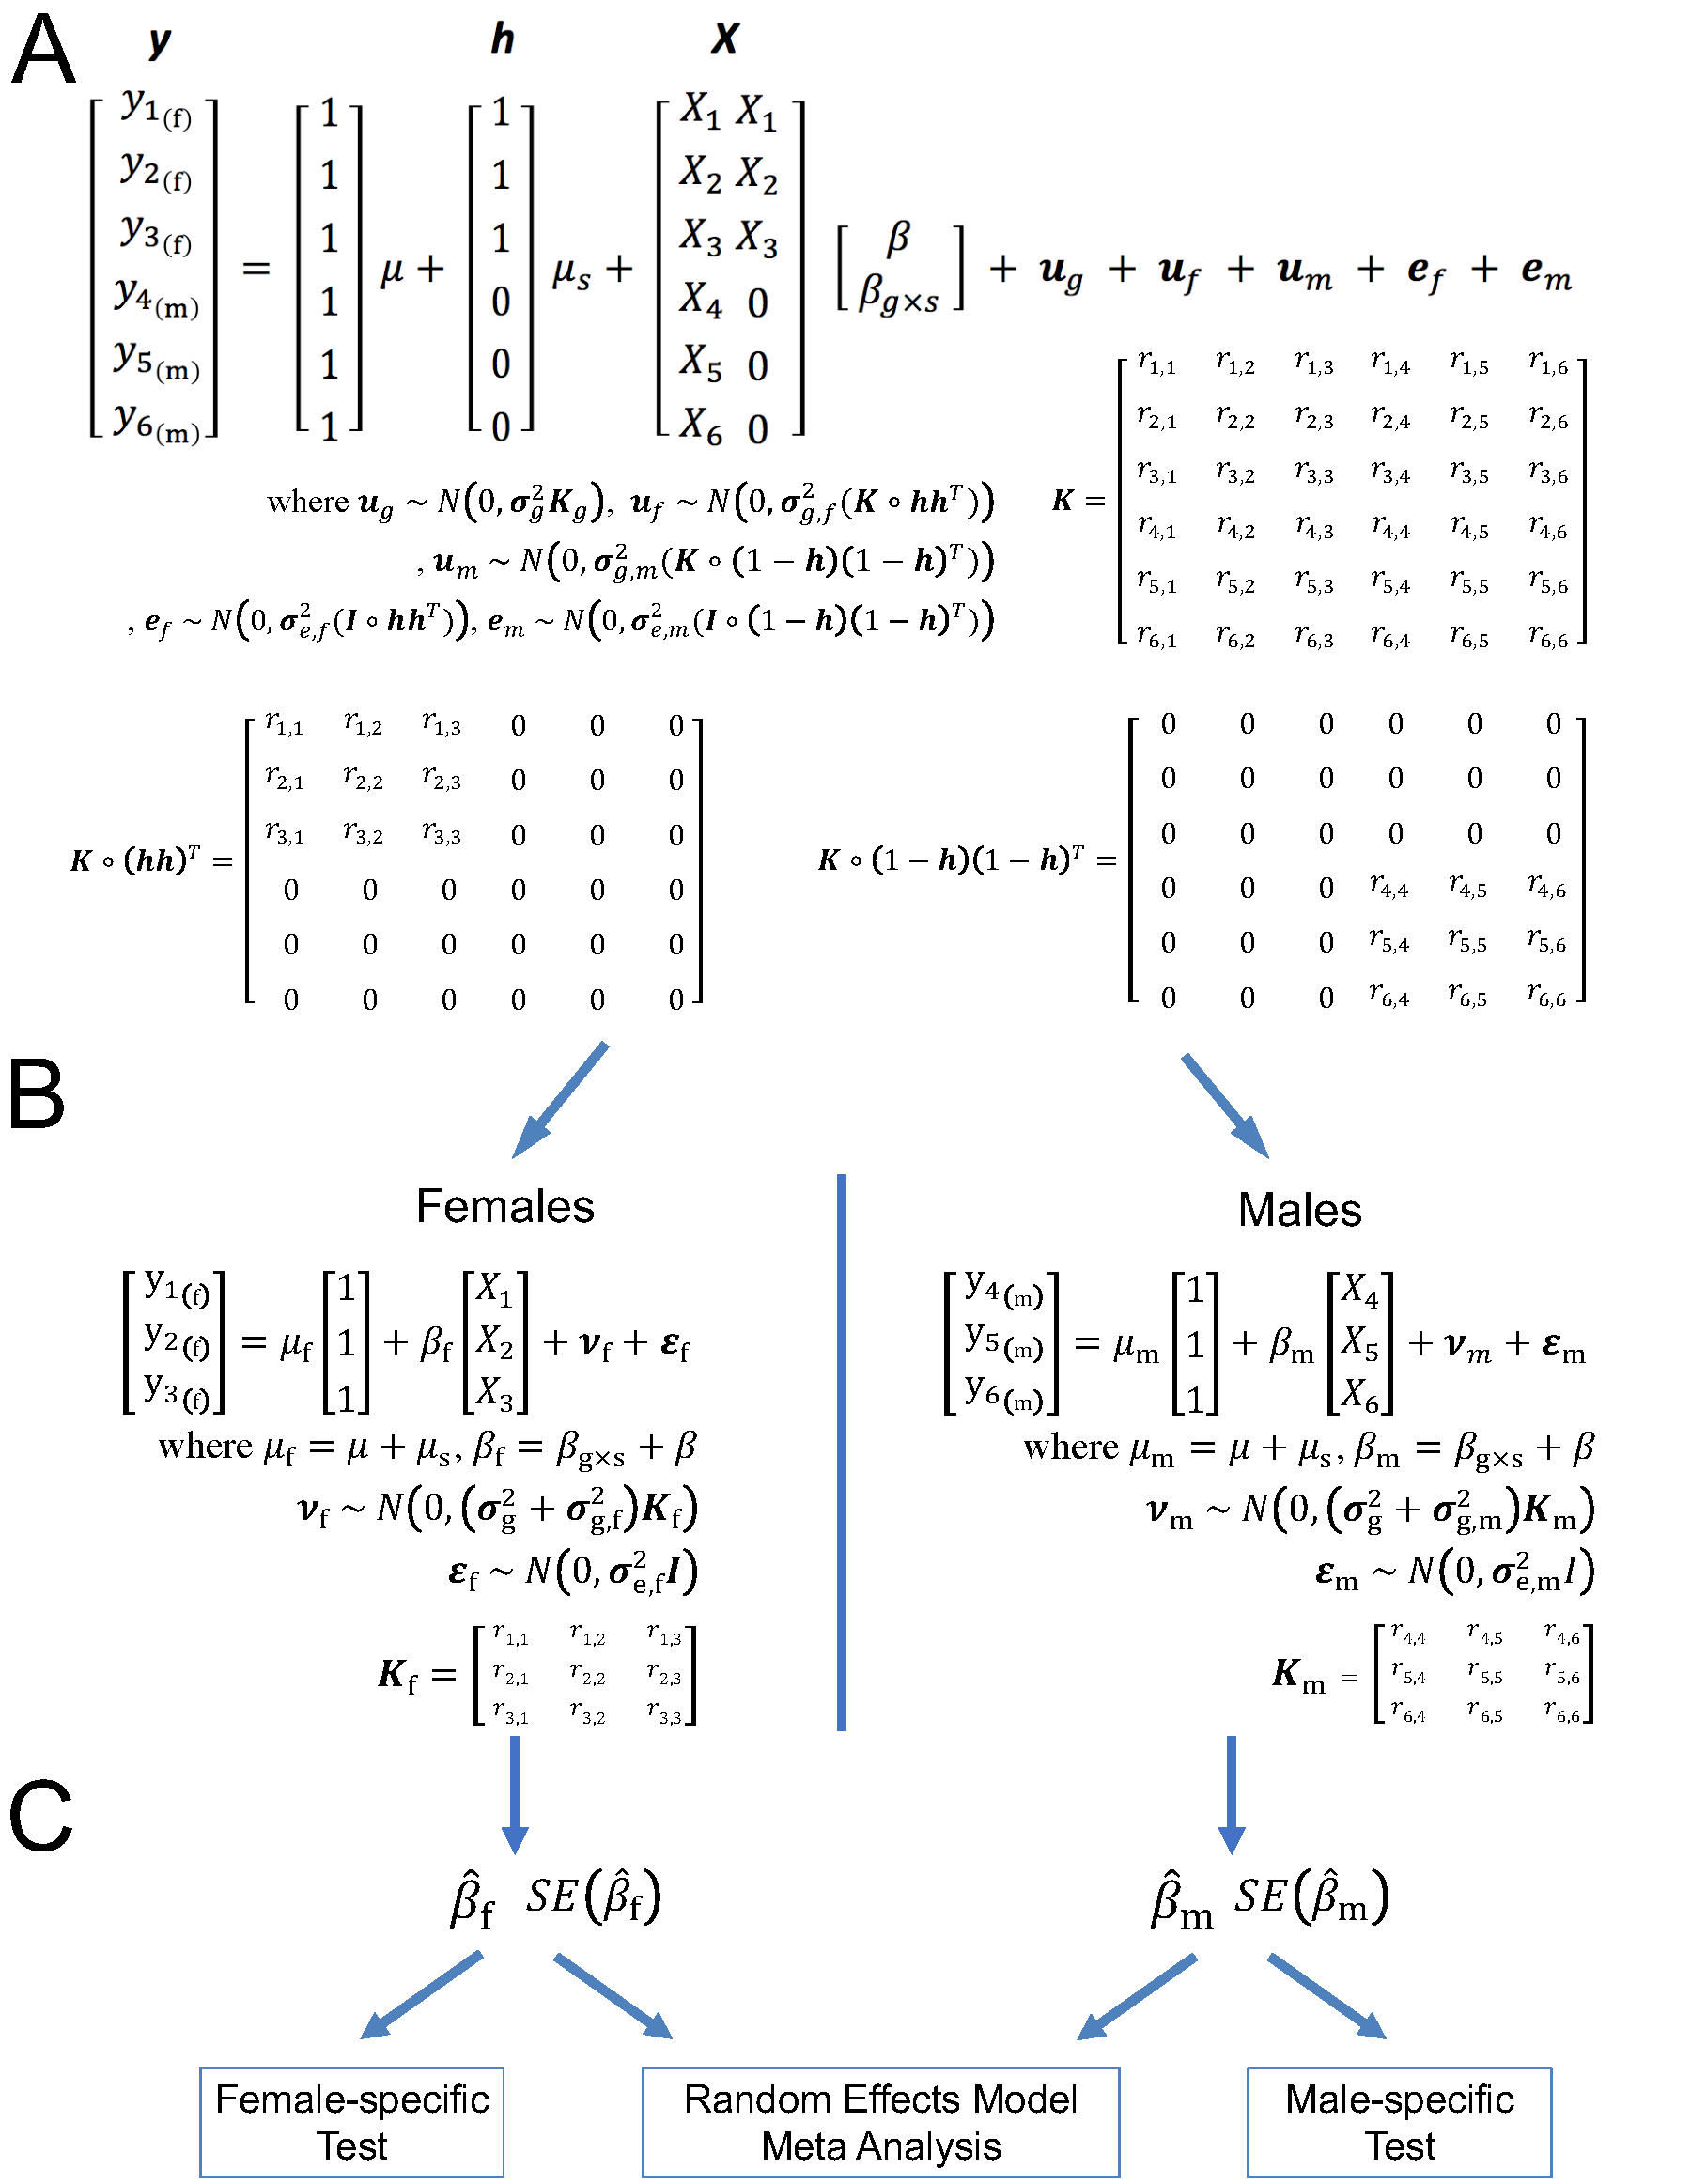
\includegraphics[width=0.96\textwidth]{../Figures/Fig1/Fig1_A4.pdf}}
  \caption{Overview of the MetaSex method.}
  \label{overview}
\end{figure}

\begin{figure}[h]
\centering
{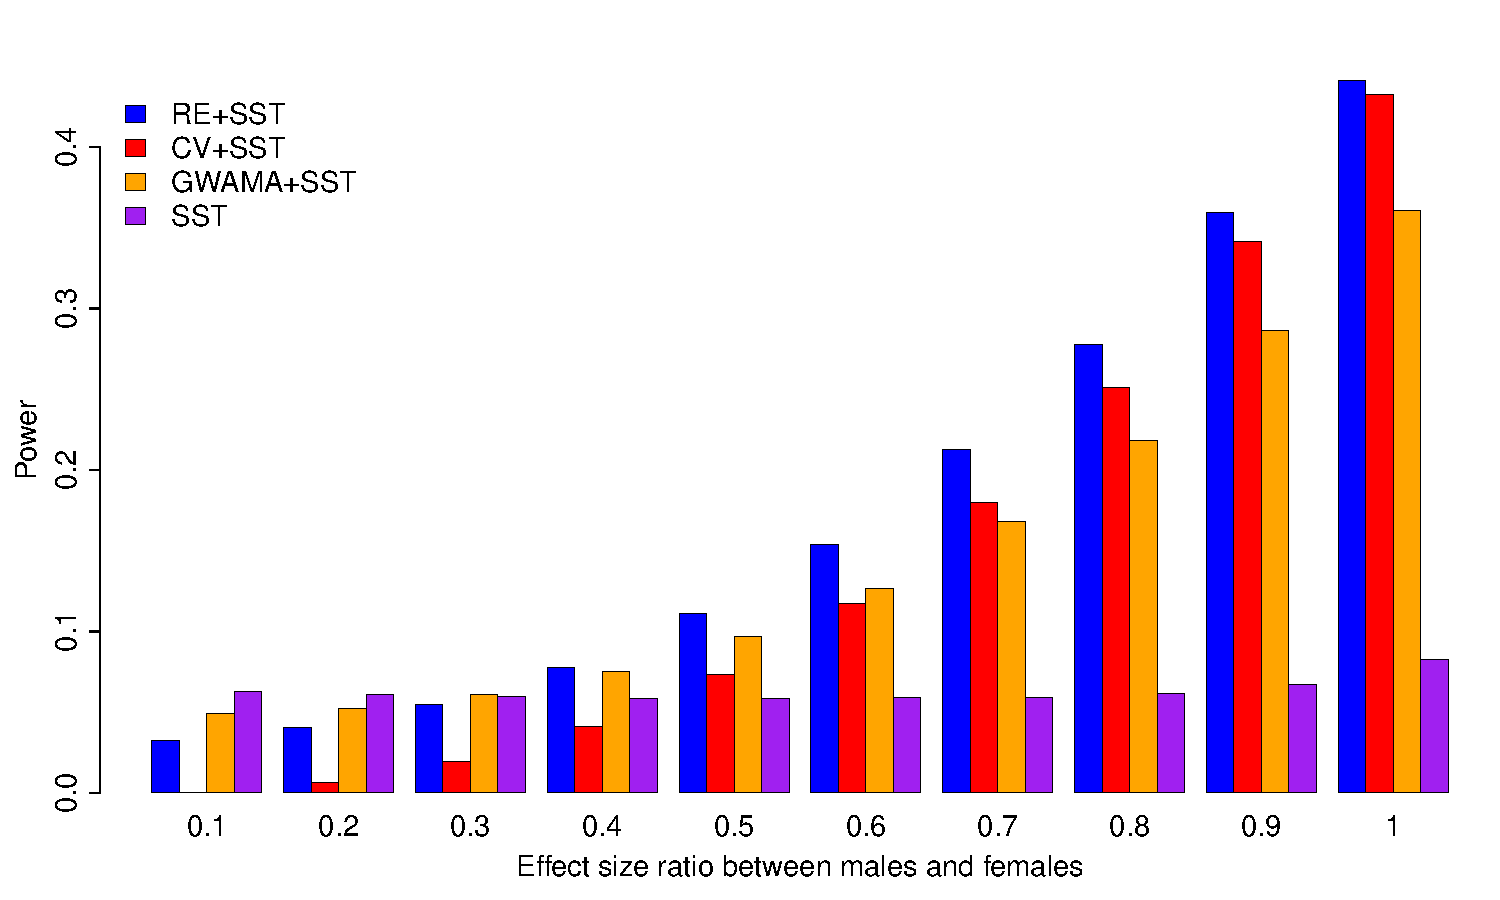
\includegraphics[width=0.96\textwidth]{../Figures/Fig2/power19_3_cv_CHL.pdf}}
\caption{ Power comparison between MetaSex (RE+SST), CV+SST, GWAMA+SST, 
and SST approaches while varying 
the effect size ratios of females and males. 
All methods were appropriately corrected for multiple testing.
}
\label{power_four}
\end{figure}

\begin{figure}[h]
\centering
{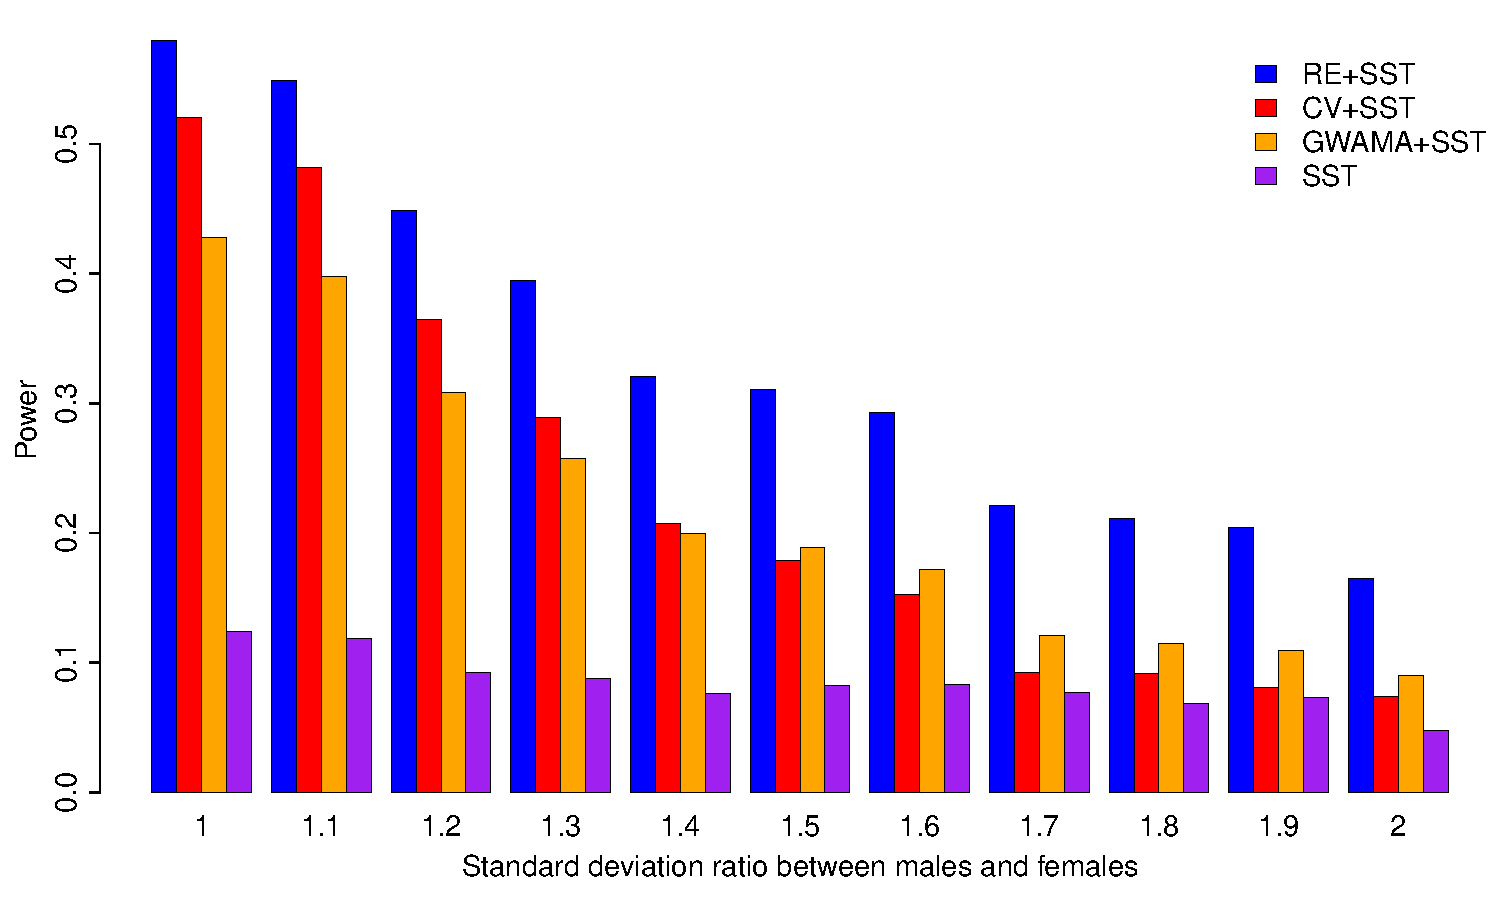
\includegraphics[width=0.96\textwidth]{../Figures/Fig3/power19_cv_res_CHL.pdf}}
\caption{ Power comparison between MetaSex (RE+SST), CV+SST, GWAMA+SST,
and SST approaches while varying 
the error variance ratio in females and males. 
%the ratio of the sex-specific standard errors of the random error term
%between female studies and male studies. 
All methods were appropriately corrected for multiple testing.
}
\label{power_res}
\end{figure}

\begin{figure}[h]
\centering
{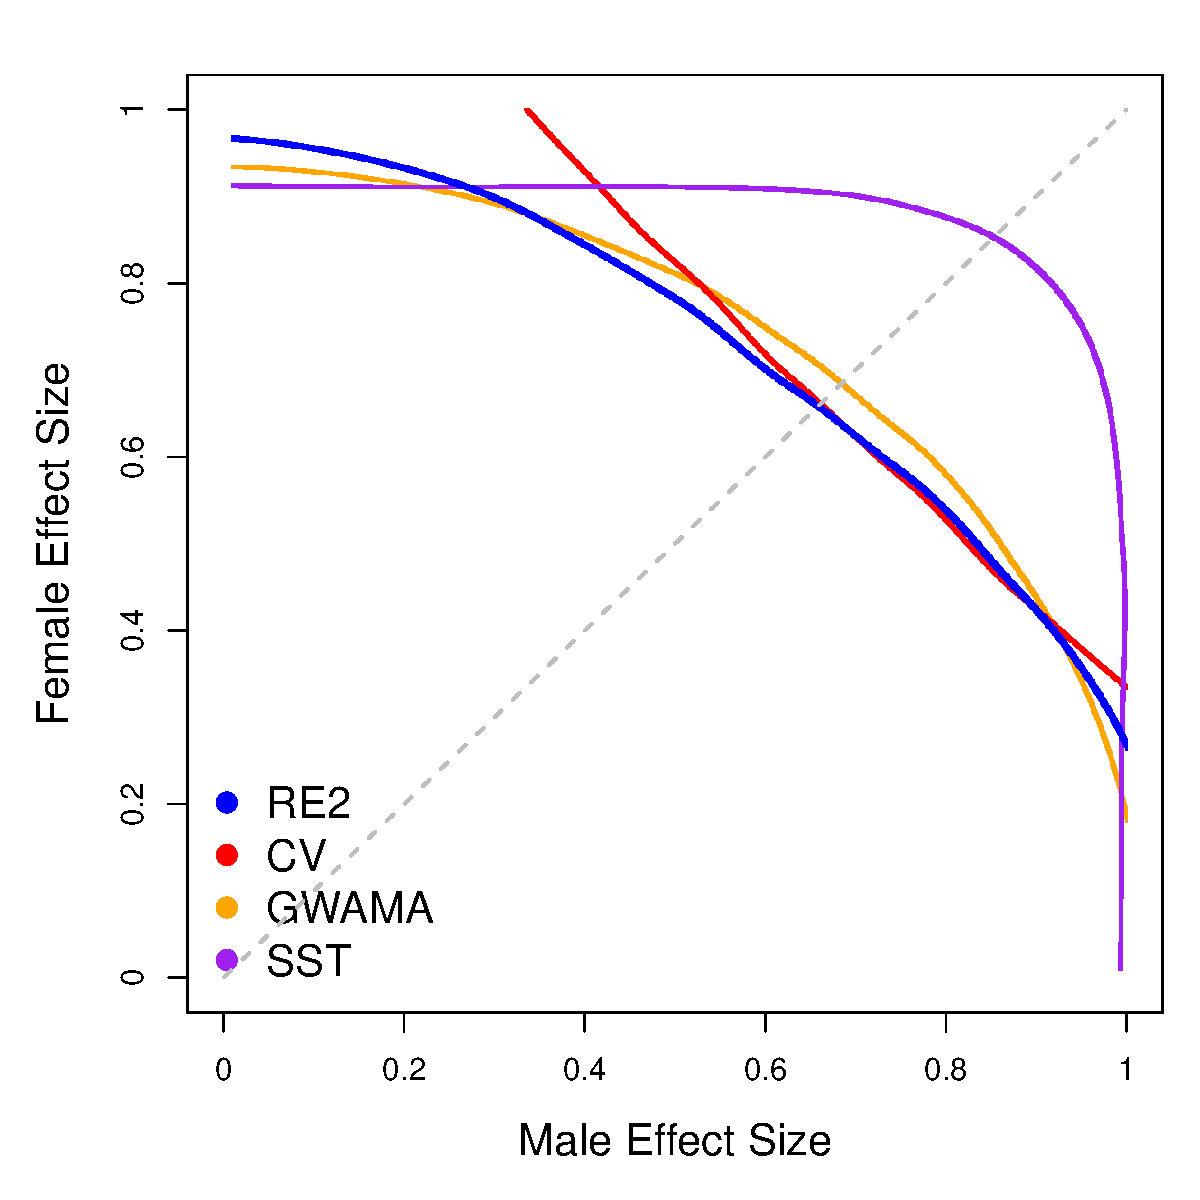
\includegraphics[width=0.96\textwidth]{../Figures/Fig4/power50_case2_CHL.pdf}}
\caption{Power characteristics of
RE, CV, GWAMA, and SST in a space 
varying the effect sizes of males and females.
%in a study consisting of an equal number of males and females.
%For the particular male and female effect size pair, 
%the simulated phenotype was generated assuming a ratio of 1.2 between sex-specific error variances
%(chosen based on NFBC data, male variance = 1.2 $\times$ female variance).
%study 
%under the assumption of balanced number of individuals. %between male and female study
%(b) and when there are twice as many females as males.
The lines denote the points where each method achieved 50\% power. 
%This figure shows the $50\%$ power lines for the four different approaches.
%Because power increases as effect size increases, the area outside of the $50\%$ power line
%(area containing the point where male effect size=1 and female effect size=1) shows the 
%area which the method achieves more than $50\%$ power.
The diagonal line shows the points where the effect sizes of the two sexes are equal.
The $50\%$ power line is skewed due to the error variance ratio of 1.2 that we assumed.
%under unbalanced number of individuals between the male and the female study.
}
\label{power_comp11}
\end{figure}

\begin{figure}[h]
  \centering
  {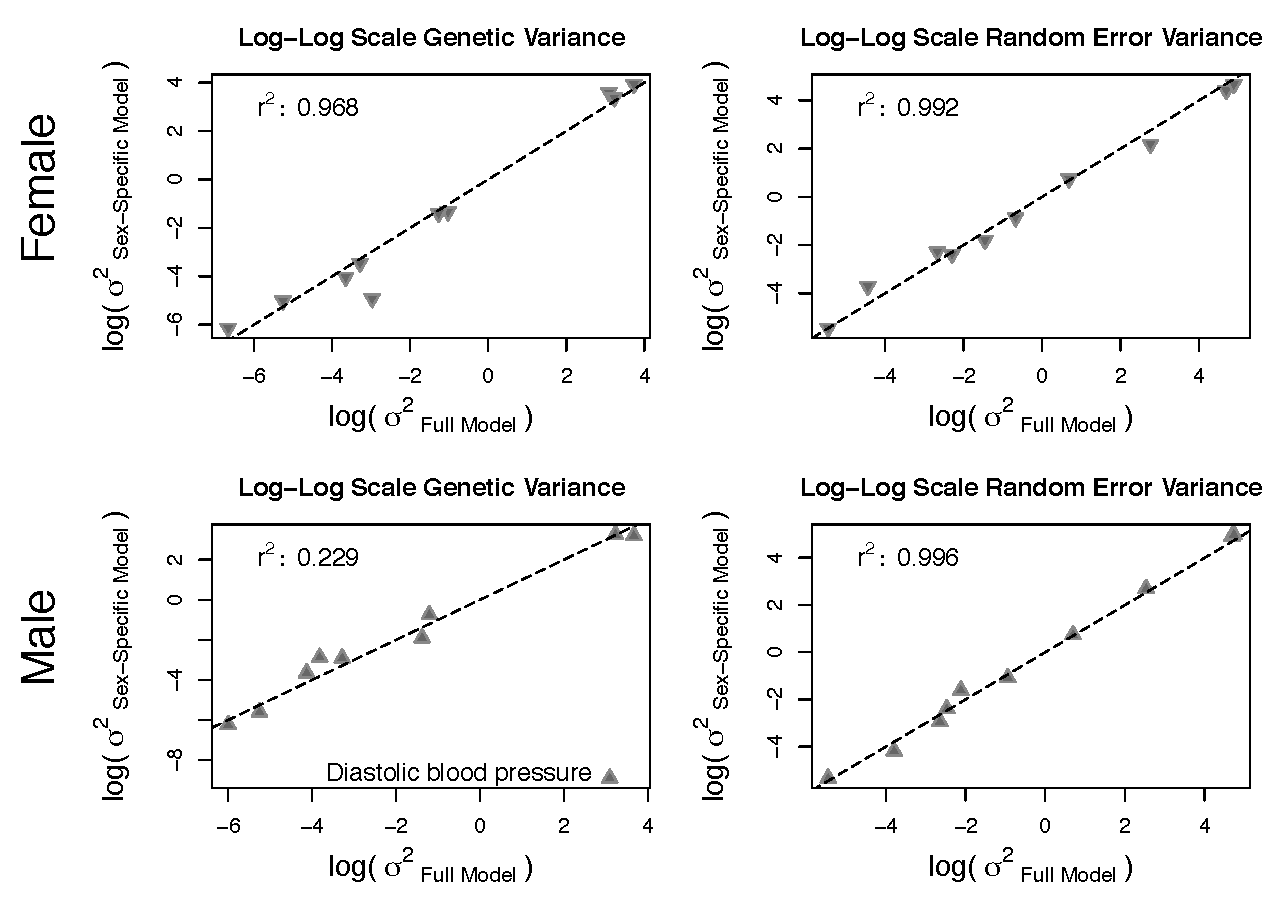
\includegraphics[width=0.96\textwidth]{../Figures/Fig5/GCTA_summary.pdf}}
  \caption{Comparison of the variance components between the full and the sex-specific
  models in 10 phenotypes of NFBC data. The points represent phenotypes and the
  dotted line is where the variance estimates of the two models are equal. We
evaluated $r^2$ in the log scale and labeled an outlier(Diastolic blood pressure) observed in the male genetic variance plot.}
  \label{gcta_summary}
\end{figure}

\begin{figure}[h!]
\centering
{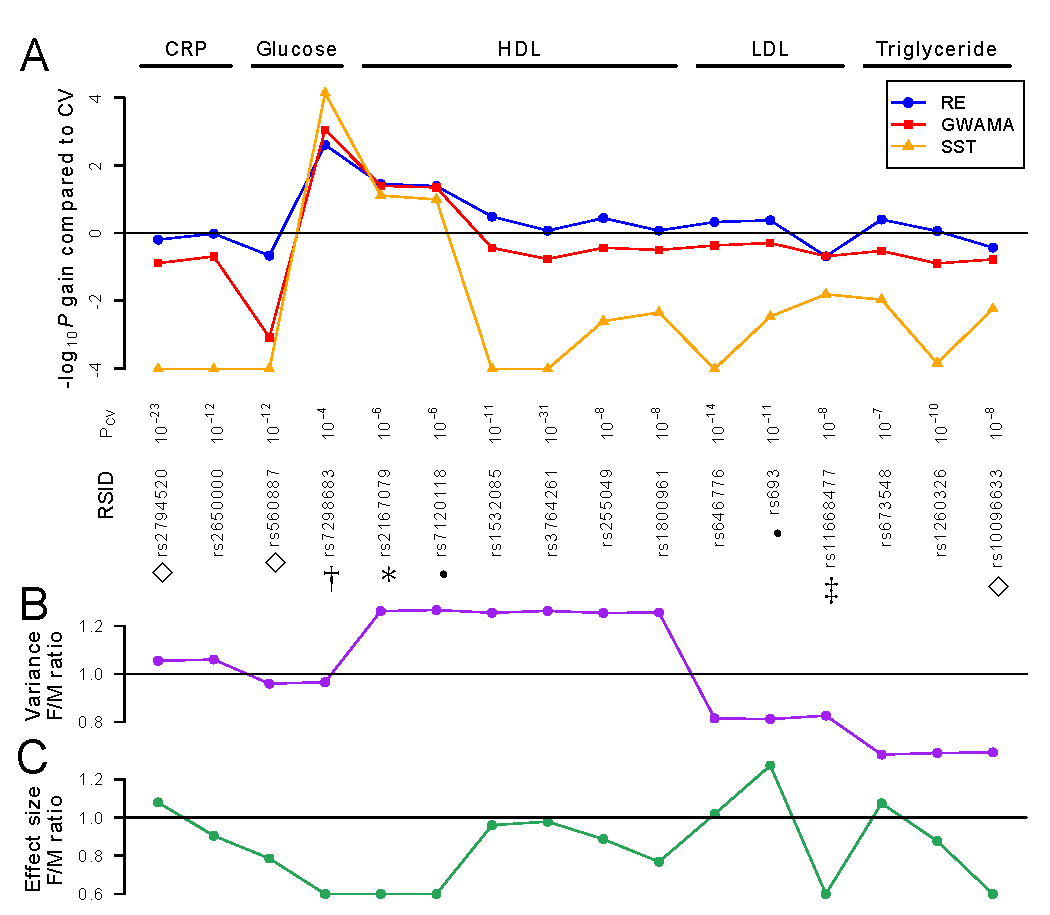
\includegraphics[width=0.96\textwidth]{../Figures/Fig6/result_plot_CHL_affinity_symbol.pdf}}
\caption{
    Association results of RE, CV, GWAMA, and SST at the 16 associated loci in 
    any of 10 phenotypes of NFBC data. 
    %Comparison of the four approaches (RE, CV, GWAMA, SST) 
%for the 16 significant loci (threshold : $5.0 \times 10^{-8}$) from
%the Northern Finland Birth Cohort data (CRP : C-reactive protein).
%If there were more than one significant locus in the same linkage disequilibrium block, we choose the most significant one. 
(A) Relative $-log_{10} \it{P}$ improvement of the other methods compared with the CV method,
namely, [$-log_{10} \it{P}$ of RE/GWAMA/SST] $-$ [$-log_{10} \it{P}$ of CV]. 
%The horizontal line represents the $-log_{10} \it{P}$ of the CV method.
The RSIDs of 16 significant SNPs as well
as their CV p-values are shown at the bottom. 
(B) The ratio of phenotypic variance between males and females after regressing out the genetic effect of each SNP.
(C) The ratio of the genetic effect size of each SNP between males and females.
}
\label{power_result}
\end{figure}
\clearpage
\beginsupplement
\section{Supplementary Tables}
%

\begin{landscape}

	
\begin{table}[p]
  \centering
  \resizebox{1\textwidth}{!}{
    \begin{tabular}{cccccccccc}
      \hline
      Phenotype & $\sigma_{g}^2(SE)$ & $\sigma_{g,f}^2(SE)$ & $\sigma_{g,m}^2(SE)$ &
      $\sigma_{e,ss}^2(SE)$ & $\sigma_{e}^2(SE)$ & $P_{g}$ & $P_{g,f}$ & $P_{g,m}$ & $P_{ss}$\\ 
      \hline

Triglyceride  & 0.0189(0.014) & 0.0323(0.0219) & 0.0031(0.0236) & 0.1134(0.0283) &
0.1205(0.0189) & $1.79^{-1}$ & $1.4^{-1}$ & $8.95^{-1}$ & $\bf{6.23^{-5}}$ \\
HDL  & 0.0375(0.0072) & 0(0.011) & 0(0.0117) & 0.0017(0.0137) & 0.0694(0.0103) &
$\bf{1.72^{-7}}$ & $1.00$ & $1.00$ & $8.99^{-1}$ \\
LDL  & 0.2569(0.0511) & 0.0237(0.0786) & 0.042(0.082) & 0.1186(0.0983) & 0.3921(0.067)
& $\bf{4.88^{-7}}$ & $7.63^{-1}$ & $6.08^{-1}$ & $2.27^{-1}$ \\
BMI  & 0.0052(0.0014) & 0(0.0022) & 0(0.0023) & 0.0107(0.0028) & 0.0118(0.002) &
$\bf{2.53^{-4}}$ & $1.00$ & $1.00$ & $\bf{1.20^{-4}}$ \\
C-reactive protein  & 0.222(0.1553) & 0.1346(0.243) & 0.0301(0.2641) & 0.0227(0.3108) &
1.9925(0.2321) & $1.53^{-1}$ & $5.80^{-1}$ & $9.09^{-1}$ & $9.42^{-1}$ \\
Glucose  & 0.0011(0.0005) & 0.0002(0.0008) & 0.0014(0.0008) & 0.0009(0.0009) &
0.0043(0.0007) & $2.31^{-2}$ & $7.83^{-1}$ & $8.66^{-2}$ & $3.56^{-1}$ \\
Insulin  & 0.0121(0.0082) & 0.0139(0.0132) & 0.004(0.0142) & 0.0163(0.0167) &
0.0847(0.0113) & $1.40^{-1}$ & $2.93^{-1}$ & $7.79^{-1}$ & $3.30^{-1}$ \\
Systolic blood pressure  & 37.1421(10.5002) & 4.5774(16.7722) & 1.9977(17.5993) &
18.3323(21.4657) & 114.189(14.6194) & $\bf{4.04^{-4}}$ & $7.85^{-1}$ & $9.10^{-1}$ & $3.93^{-1}$ \\
Diastolic blood pressure  & 22.0399(8.3115) & 0.0001(12.9059) & 0.0001(13.6516) &
11.6098(16.1558) & 97.5402(11.0647) & $8.01^{-3}$ & $1.00$ & $1.00$ & $4.72^{-1}$ \\
Height  & 24.0673(2.6501) & 1.2284(3.8886) & 1.1577(4.2184) & 3.2263(4.9783) &
12.6085(3.326) & $\bf{1.07^{-19}}$ & $7.52^{-1}$ & $7.84^{-1}$ & $5.17^{-1}$ \\

\hline
\end{tabular}
   }
\caption {Variance components of 10 NFBC phenotypes in the full five-variance-component model. 
  For each trait, we tested if the variance of the polygenic background effect term($\sigma_{g}^2$) is significantly non-zero ($P_{g}$) and if the variance of
  sex-specific error term($\sigma_{e,ss}^2$) is significantly non-zero ($P_{ss}$). 
  The p-values less than the 0.005 are in bold font. 
}


\label{finland_gcta_withP}
\end{table}

\end{landscape}


\begin{table}[h!]
%\tiny
\centering
\resizebox{0.75\textwidth}{!}{
\begin{tabular}{cccccc}
\hline
Phenotype &  SST(F)   & SST(M)       &     RE           &   CV      &   GWAMA          \\
\hline
Triglyceride  &   1.007 & 0.991  &  0.995 &   1.001 &    1.006    \\
HDL  &  1.002 & 0.995  & 1.008 &   1.003 &     0.993    \\
LDL  &  1.001 &  0.996   & 1.011 &   1.002 &     1.004   \\
BMI  &  0.999 & 0.996  &  0.992 & 0.994 &     0.994    \\
C-reactive protein   &  0.994 &  0.989  &  0.998 &   0.993  &    0.994    \\
Glucose  &  1.006 &  1.000   &  1.011 &    1.008  &   1.006     \\
Insulin  &  1.004 &  0.996  &  1.006 &   1.005  &     1.001   \\
Systolic blood pressure  &  0.997 &  0.997 &  1.012 &   1.006  &   1.000     \\
Diastolic blood pressure  &  0.998 & 1.008  & 1.013 &   1.006  &   1.002     \\
Height  &  1.004 & 1.002  &  1.028 &   1.003  &    1.001    \\
\hline
\end{tabular}
}
\caption{ Genomic control factor in the genome-wide association mapping of 10 NFBC phenotypes.
   % \hl{You can similarly change trait names here, too.}
 }
\label{finland_lambda1}
\end{table}




\begin{table}
\footnotesize
\centering
\resizebox{0.899\textwidth}{!} {
\begin{tabular*}{1.11\textwidth}  {@{\extracolsep{\fill}} |c|c|c|c|c|c|c|c|c|}
\hline
\multicolumn{4}{|c|}{\textbf{Phenotype : C-reactive protein }} &  \multicolumn{2}{c|}{\textbf{sex-specific}} &  \multicolumn{2}{c|}{\textbf{beta$\pm$std error}}  &  \textbf{best} \\
\hline
\textbf{rsid}   &  \textbf{RE}  & \textbf{CV}  & \textbf{GWAMA}   & \textbf{SST(F)}   & \textbf{SST(M)} &  \textbf{female}   & \textbf{male} & \textbf{methods} \\
\hline
\hline
rs2794520 &   3.32e-23 & \textbf{2.11e-23} &  1.64e-22         & 1.28e-13 & 2.93e-11  &   0.314$\pm$0.042 & 0.291$\pm$0.043  & RE,CV\\ 
rs2650000 &  \textbf{1.71e-12} & 1.64e-12 &   8.09e-12        & 2.79e-06 & 8.65e-08   &  0.199$\pm$0.042 & 0.220$\pm$0.041 & RE,CV \\ 
%Chr17:68989647 & rs7406617 & 0.00011 & \textbf{3.61e-06} & 8.15e-05 & 8.11e-05 & 1.66e-07 & 0.88493 & -0.251$\pm$0.048 & -0.006$\pm$0.049 & RE \\ 
\hline
\hline
\multicolumn{4}{|c|}{\textbf{Phenotype : Glucose  }} &  \multicolumn{2}{c|}{\textbf{sex-specific}}  & \multicolumn{2}{c|}{\textbf{beta$\pm$std error}} & \textbf{best} \\
\hline
\textbf{rsid}   & \textbf{RE}  & \textbf{CV}  & \textbf{GWAMA}    & \textbf{SST(F)}   & \textbf{SST(M)}    & \textbf{female}   & \textbf{male} & \textbf{methods} \\
\hline
\hline
rs560887 &   5.30e-12 & \textbf{1.14e-12} &    1.39e-09       & 8.19e-06 & 4.83e-08 &    0.011$\pm$0.002 & 0.014$\pm$0.002  & CV \\ 
%Chr7:15030358 & rs10244051 & 2.14e-07 &  2.61e-07 & \textbf{1.74e-07} & 1.77e-07 & 0.00029 & 0.00021 & -0.007$\pm$0.002 & -0.007$\pm$0.002  & FE,RE,CV,CM \\ 
%Chr11:92362409 & rs1447352 & 1.31e-07 &  1.59e-07 & 9.07e-08 & \textbf{8.72e-08} & 0.00037 & 9.46e-05 & 0.007$\pm$0.002 & 0.007$\pm$0.002 & FE,RE,CV,CM \\ 
%Chr11:92363999 & rs7121092 & 1.32e-07 &  1.59e-07 & 9.53e-08 & \textbf{9.12e-08} & 0.00031 & 0.00011 & 0.007$\pm$0.002 & 0.007$\pm$0.002  & FE,RE,CV,CM  \\ 
rs7298683 &   2.01e-07 & 8.14e-05  &      7.23e-08       &   0.86718 & \textbf{5.92e-09} &      -0.0007$\pm$0.004 & 0.026$\pm$0.004 & SST(M) \\ 
\hline
\hline
\multicolumn{4}{|c|}{\textbf{Phenotype : HDL   }} &  \multicolumn{2}{c|}{\textbf{sex-specific}}   & \multicolumn{2}{c|}{\textbf{beta$\pm$std error}} & \textbf{best} \\
\hline
\textbf{rsid}   &  \textbf{RE}  & \textbf{CV}   & \textbf{GWAMA}    & \textbf{SST(F)}   & \textbf{SST(M)}    & \textbf{female}   & \textbf{male} & \textbf{methods}  \\
\hline
\hline
%Chr2:21047434 & rs6728178 & \textbf{2.19e-07} & 2.68e-07 & 4.52e-07 & 4.54e-07 & 0.00390 & 1.16e-05 & -0.031$\pm$0.011 & -0.043$\pm$0.010 &  FE,RE  \\
%Chr8:19875201 & rs10096633 & 4.74e-07 & \textbf{4.62e-07} & 2.66e-06 & 2.69e-06 & 0.04291 & 6.66e-07 & -0.034$\pm$0.017 & -0.074$\pm$0.015 & FE,RE  \\
rs2167079 &  \textbf{4.46e-08} & 1.26e-06 &     5.06e-08       &0.01838 & 9.78e-08 &     -0.024$\pm$0.010 & -0.055$\pm$0.010 &  RE, GWAMA \\
rs7120118 &  \textbf{4.62e-08} & 1.13e-06  &    5.07e-08      & 0.01679 & 1.15e-07 &     -0.024$\pm$0.010 & -0.054$\pm$0.010 &  RE, GWAMA \\
 rs1532085 &  \textbf{3.53e-12} & 1.08e-11  &    2.98e-11       &1.87e-06 & 2.25e-07 &     -0.048$\pm$0.010 & -0.050$\pm$0.009 & RE  \\
 rs3764261 &  \textbf{4.15e-32} & 4.89e-32  &    2.88e-31      & 8.85e-16 & 3.63e-18 &    -0.090$\pm$0.011 & -0.092$\pm$0.010 & RE,CV \\
 rs255049 &  \textbf{5.26e-09} & 1.45e-08  &    3.94e-08       &0.00014 & 5.85e-06 &     -0.047$\pm$0.012 & -0.053$\pm$0.011 & RE  \\
 rs1800961 &  \textbf{2.39e-08} & 2.82e-08  &    8.96e-08       &0.00051 & 6.29e-06 &     0.083$\pm$0.023 & 0.108$\pm$0.023 & RE,CV \\
\hline
\hline
\multicolumn{4}{|c|}{\textbf{Phenotype : LDL  }} &  \multicolumn{2}{c|}{\textbf{sex-specific}}   & \multicolumn{2}{c|}{\textbf{beta$\pm$std error}} & \textbf{best}  \\
\hline
\textbf{rsid}   & \textbf{RE}  & \textbf{CV}  & \textbf{GWAMA}    & \textbf{SST(F)}   & \textbf{SST(M)}   & \textbf{female}   & \textbf{male} & \textbf{methods}  \\
\hline
\hline
 rs646776 &  \textbf{1.97e-15} & 4.17e-15 &     9.71e-15      & 8.36e-10 & 2.11e-07 &    0.169$\pm$0.027 & 0.166$\pm$0.031 & RE \\
%Chr1:205941798 & rs4844614 & \textbf{1.27e-07} & 1.52e-07 & 2.52e-07 & 2.52e-07 & 0.00080 & 2.78e-05 & -0.080$\pm$0.024 & -0.113$\pm$0.027 &  FE,RE,CV,CM \\
rs693 &  \textbf{1.25e-11} & 2.97e-11 &    5.84e-11      & 8.81e-09 &  0.00013    &    -0.131$\pm$0.022 & -0.103$\pm$0.026 & RE \\
 rs11668477 &  1.98e-08 & \textbf{4.04e-09} &    1.96e-08       & 0.00240 & 2.62e-07 &    0.090$\pm$0.029 & 0.179$\pm$0.034 & CV \\
%Chr19:50087106 & rs157580 & \textbf{3.18e-07} & 3.86e-07 & 3.24e-07 & 3.25e-07 & 9.62e-06 & 0.00682 & 0.110$\pm$0.025 & 0.075$\pm$0.028 & FE,RE,CV,CM  \\
\hline
%\hline
%\multicolumn{6}{|c|}{\textbf{Phenotype : sysres  }} &  \multicolumn{2}{c|}{\textbf{sex-specific}} &  \multicolumn{2}{c|}{\textbf{beta$\pm$std error}} & \textbf{best}  \\
%\hline
%\textbf{Position}  & \textbf{rsid}   & \textbf{FE} & \textbf{RE}  & \textbf{Covariate}   & \textbf{Combined}   & \textbf{female}   & \textbf{male}   & \textbf{female}   & \textbf{male} & \textbf{methods}   \\
%\hline
%\hline
%Chr2:55702813 & rs782602 & \textbf{7.30e-08} & 8.55e-08 & 1.42e-07 & 1.42e-07 & 6.00e-06 & 0.00246 & 1.555$\pm$0.343 & 1.115$\pm$0.368 & FE,RE,CV,CM  \\
%Chr7:33208521 & rs10486523 & 5.47e-07 & 6.67e-07 & 4.95e-07 & \textbf{4.94e-07} & 0.00027 & 0.00059 & -2.351$\pm$0.646 & -2.435$\pm$0.710 &  FE,RE,CV,CM \\
%\hline
\hline
\multicolumn{4}{|c|}{\textbf{Phenotype : Triglyceride  }} &  \multicolumn{2}{c|}{\textbf{sex-specific}}   & \multicolumn{2}{c|}{\textbf{beta$\pm$std error}} & \textbf{best}  \\
\hline
\textbf{rsid}   &  \textbf{RE}  & \textbf{CV} & \textbf{GWAMA}    & \textbf{SST(F)}   & \textbf{SST(M)}    & \textbf{female}   & \textbf{male} & \textbf{methods}  \\
\hline
\hline
 rs673548 & \textbf{2.61e-08} & 6.54e-08 &     2.21e-07       &6.11e-06 & 0.00097 &  0.058$\pm$0.012 & 0.054$\pm$0.016 & RE \\
rs1260326 & \textbf{1.64e-10} & 1.88e-10 &     1.49e-09      & 1.32e-06 & 2.10e-05 &     -0.057$\pm$0.011 & -0.065$\pm$0.015 & RE,CV \\
 rs10096633 &  5.32e-08 & \textbf{1.98e-08} &   1.19e-07        & 0.00109 & 3.47e-06 &   0.062$\pm$0.019 & 0.113$\pm$0.024 & CV  \\
\hline
\end{tabular*}
}
\caption{ Association mapping results of the NFBC data. 
    %Comparison of different approaches in the Northern Finland Birth Cohort data. 
The SNPs are presented for which any method gave $P < 5\times 10^{-8}$ in any of 10 phenotypes.
%After correcting with genomic control,
%if any $\textit{p-value}$ from any approach is significant 
%(threshold: $5.0 \times 10^{-8}$)
%(threshold RE+SST : $2.39 \times 10^{-8}$, 
%FE, Covariate, Combined : $5 \times 10^{-8}$), 
%then we include this result in the table. 
For each SNP, the most significant p-value among the four methods (RE, CV, GWAM, and SST)
is in bold font. 
The ``beta'' column shows the effect sizes of male- and female-only studies and their estimated standard errors.
For each significant association, we report the ``best methods'', 
the set of methods whose p-value was less than two times the most significant 
p-value for each association.
%For example, for the association at rs1532085 in the HDL phenotype, 
%the most significant p-value is $2.93 \times 10^{-12}$ . 
%However, the p-value for the CV method ($1.01 \times 10^{-11}$) and 
%the GWAMA method ($3.39 \times 10^{-11}$) are greater than 
%twice that value. %$7.92 \times 10^{-8}$.
%Thus, only RE is included in the best methods for this SNP.
%To get an overall comparison of the relative power of the approaches, we compare the 
%number of times the each approach is selected as the best methods. 
%For the six NFBC phenotypes with significant associations, 
%the RE approach is the best methods for 12 associated loci whereas
%the CV approach is the best methods for 8 associated loci and the 
%GWAMA approach is the best methods for only 2 associated loci.
%The SST approach is the best method for only one associated locus. 
}
\label{tab:NFBC1}
\end{table}




\end{document}
